\section{Simulación del prototipo}

Las condiciones de simulación y ensayo fueron:

\begin{itemize}
    \item Tensión de entrada: $V_s=36V$
    \item Frecuencia de conmutación: $f=125kHz$
    \item Ciclo de trabajo: $D=0.4$
    \item Resistencia de carga: $R=88.5\Omega$
\end{itemize}

% % 1) Tensión de salida en el colector del TL494 <<< DONE

% Se verifica que el ciclo de trabajo es de $D=0.4$ y la frecuencia de conmutación es de aproximadamente $f=125kHz$. 
% Su amplitud se reduce considerablemente de los $12V$ que poseía sin la carga del convertidor a $8V$ con el mismo acoplado. 
% La forma de onda presenta una leve deformación respecto a la señal sin carga. 

% % 2) Tensión en el capacitor Ct <<< N/A <<< DONE

% Se observa una disminución en la frecuencia de la forma de onda a aproximadamente $f=112kHz$. 
% El prototipo presenta una oscilación no deseada de $f_{osc}=1.25MHz$, 
% la cual estará presente en muchas de las formas de onda que se analizarán a continuación. 

% % 3) Tensión de salida de la etapa de ganancia de corriente <<< DONE

% Dado que la etapa posee ganancia de tensión unitaria, su forma de onda es aproximadamente igual a la tensión de salida del TL494. 
% Las oscilaciones fueron eliminadas mediante la red snubber. 

% % 4) Tensión en el primario del transformador del driver <<< DONE

% La amplitud y la forma de onda de la señal del prototipo coinciden respecto a la simulación. 
% Se observan unos picos en los flancos de subida y de bajada. 

% % 5) Tensión en el secundario del transformador del driver <<< DONE

% La amplitud y la forma de onda de la señal del prototipo coinciden respecto a la simulación. 
% Se observa un pico en el flanco de bajada. 

% % 6) Corriente en el primario del transformador del driver <<< DONE

% La forma de onda del prototipo está deformada y posee levemente mayor amplitud. 

% % 7) Corriente en la resistencia entre gate y source del driver <<< DONE

% La amplitud y la forma de onda de la señal del prototipo coinciden respecto a la simulación. 
% Presenta la oscilación de $f_{osc}=1.25MHz$. 

% % 8) Corriente que circula por el gate del MOSFET 1 (high side)

% El prototipo presenta una segunda onda triangular negativa indeseada. 
% Además, sus picos de amplitud son mayores. 

% % 9) Corriente que circula por el gate del MOSFET 2 (low side)

% El prototipo presenta un pico negativo indeseado. 
% Presenta la oscilación de $f_{osc}=1.25MHz$. 

% % 10) Corriente que circula por el drain del MOSFET 1 (high side) <<< DONE

% La amplitud del prototipo es 1A menor respecto a la simulada debido a que las puntas de corriente desacoplan la continua. 

% % 11) Corriente que circula por el drain del MOSFET 2 (low side) <<< DONE

% La amplitud del prototipo es 1A menor respecto a la simulada debido a que las puntas de corriente desacoplan la continua. 

% % 12) Corriente en el primario del transformador de potencia 

% La amplitud del prototipo es menor respecto a la simulada debido a que las puntas de corriente desacoplan la continua. 

% % 13) Corriente en el inductor del filtro de salida 

% La amplitud de la forma de onda del prototipo es 30mA menor a la simulada. 
% Además, presenta una oscilación de $f=3.68MHz$ en la rampa de subida y de $f=38.5MHz$ en la de bajada. 

% % 14) Corriente por la carga y su ripple
% % Revisar valor

% Su amplitud es 30mA menor a la simulada y presenta una oscilación de $f=34MHz$.

% % 15) Tensión entre gate y source del MOSFET 1 (high side)

% La amplitud y la forma de onda de la señal del prototipo coinciden respecto a la simulación.
% Presenta la oscilación de $f_{osc}=1.25MHz$. 

% % 16) Tensión entre drain y source del MOSFET 1 (high side)

% Exceptuando el pico, la amplitud y la forma de onda de la señal del prototipo coinciden respecto a la simulación.
% Presenta la oscilación de $f_{osc}=1.25MHz$. 

% % 17) Tensión entre gate y source del MOSFET 2 (low side)
% % REPETIDA

% Es la tensión de salida de la etapa de ganancia de corriente.

% % 18) Tensión entre drain y source del MOSFET 2 (low side)

% Exceptuando el pico, la amplitud y la forma de onda de la señal del prototipo coinciden respecto a la simulación.
% Presenta la oscilación de $f_{osc}=1.25MHz$. 

% % 19) Tensión en el primario del transformador de potencia 

% La forma de onda del prototipo difiere de la simulada. 
% Tiene un pico en el flanco de bajada. 
% Presenta la oscilación de $f_{osc}=1.25MHz$. 

% % 20) Tensión en el secundario del transformador de potencia 
% % ADJUNTAR AMBAS IMÁGENES 

% Con una relación 1:1, la tensión en el secundario era de 44V, mucho menor a la tensión en el primario. 
% Con una relación 1:2, la tensión en el secundario es de 68V, aproximadamente igual a la del primario.
% Presenta oscilaciones de $f_{osc_{1}}=3.23MHz$ en la subida y en la bajada y de $f_{osc_{2}}=2.63MHz$ anterior a la subida. 

% % 21) Tensión de salida sobre la carga y su ripple 

% El ripple del prototipo es de 80mV fino y 200mV grueso. 
% Luego de 120mV. Presenta una oscilación de 2MHz. 

% % 22) Tensión en el inductor del filtro de salida

% El prototipo presenta una oscilación de $f_{osc}=3.03MHz$. 

% % 23) Corriente de salida por colector del TL494 
% % 24) Tensión cátodo ánodo en el diodo D1
% % 25) Tensión cátodo ánodo en el diodo D2
% % 26) Tensión cátodo ánodo en el diodo D3

% El prototipo presenta una oscilación de $f_{osc}=3.03MHz$. 

% % 27) Tensión cátodo ánodo en el diodo D4

% El prototipo presenta una oscilación de $f_{osc}=3.03MHz$. 

% % 28) Corriente en el secundario del transformador de potencia

% El prototipo presenta una oscilación de $f_{osc}=5.26MHz$.

\subsection{Generador de señal PWM}

No se realizarán comparaciones ya que su circuito no fue simulado debido a la ausencia de un correcto modelo del TL494.
El mismo fue implementado primero en una protoboard y luego en un circuito impreso.
Sus formas de onda más importantes se compararán con las indicadas en la hoja de datos del fabricante.

En la figura \ref{fig:osc_pwm_vout_disconnected} se observa la tensión a la salida del TL494 medida del prototipo.

\begin{figure}[H]
    \centering
    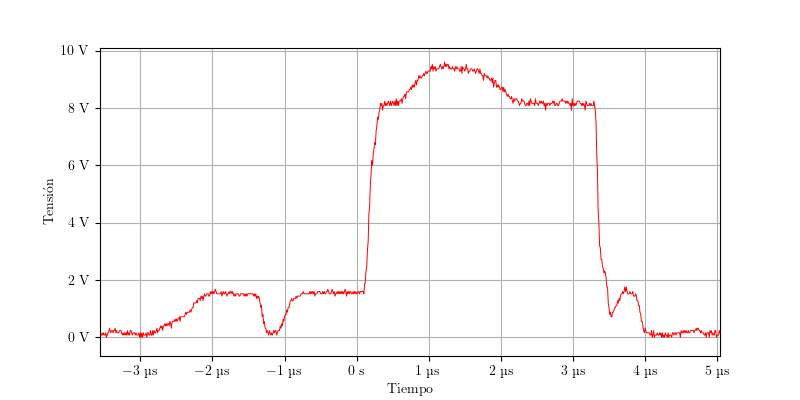
\includegraphics[width=0.8\textwidth]{images/capturas-osciloscopio/17-11-2022/1.png}
    \caption{Tensión a la salida del TL494}
    \label{fig:osc_pwm_vout_disconnected}
\end{figure}

% Se verifica que el ciclo de trabajo es de $D=0.4$ y la frecuencia de conmutación es de aproximadamente $f=125kHz$. 
% Su amplitud se reduce considerablemente de los $12V$ que poseía sin la carga del convertidor a $8V$ con el mismo acoplado. 
% La forma de onda presenta una leve deformación respecto a la señal sin carga. <<< Comparando con otras formas de onda, esta está casi identica
Se puede observar que la señal cumple con los requisitos de frecuencia ($f=125kHz$) y ancho de pulso ($D=0.4$).
La amplitud de la señal es de $8V$, lo cual es menor a la señal sin carga ($12V$).
Durante la implementación se presentaron oscilaciones de alta frecuencia durante el ciclo de apagado de la señal PWM, las cuales son tratadas en la sección \ref{subsec:oscilaciones}.
En la figura \ref{fig:sim:osc_pwm_vout} se muestra la misma forma de onda simulada en LTspice.

\begin{figure}[H]
    \centering
    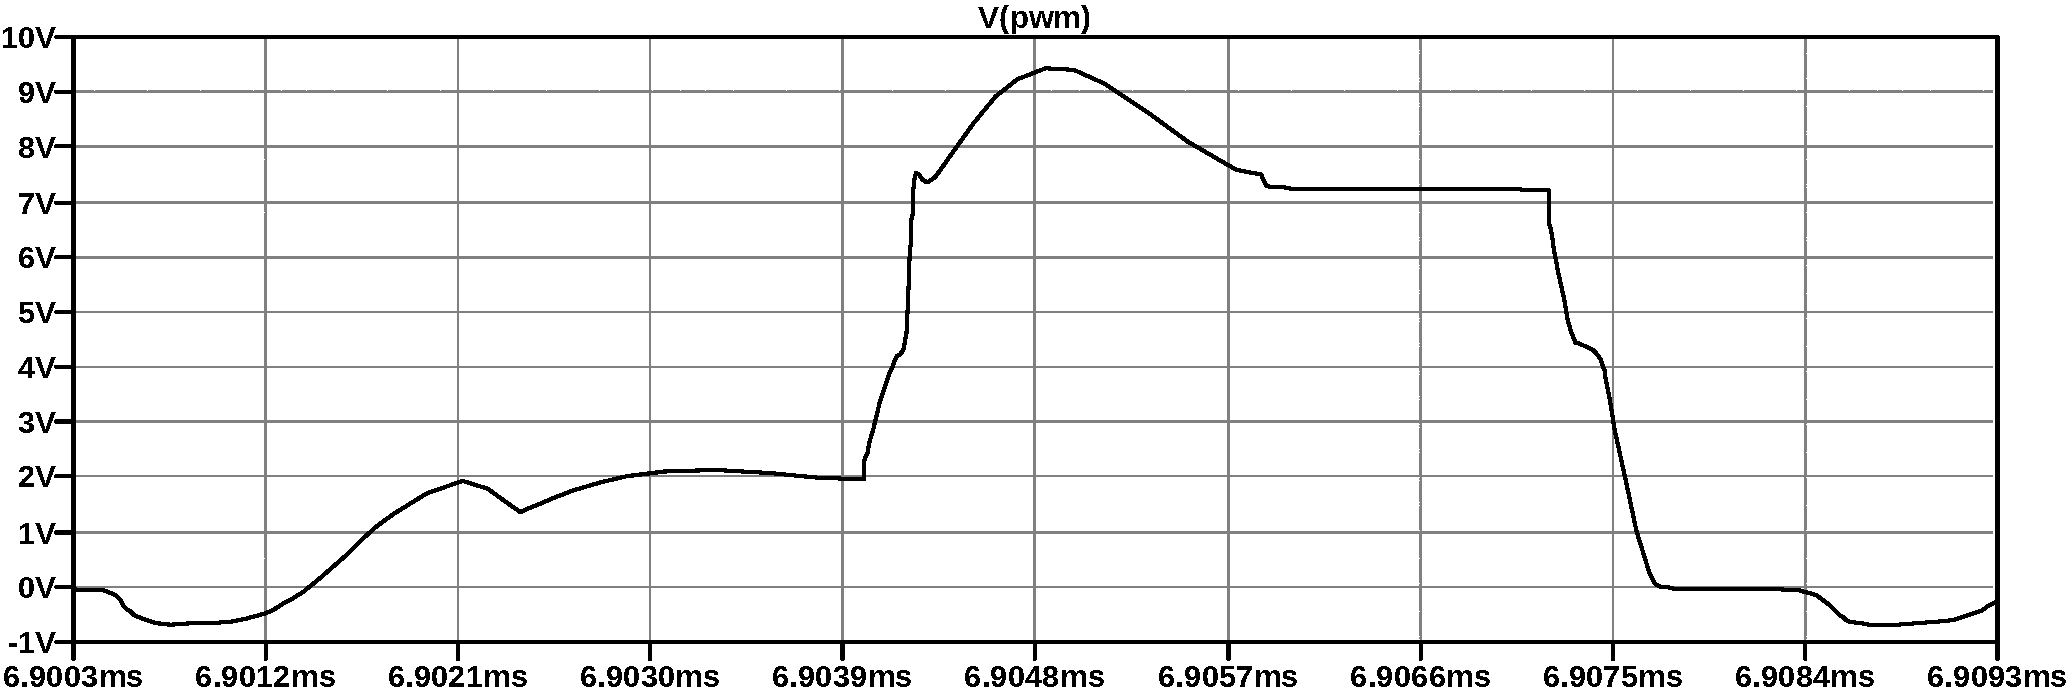
\includegraphics[width=\textwidth]{images/sim/3.pdf}
    \caption{Simulación de la tensión a la salida del TL494}
    \label{fig:sim:osc_pwm_vout}
\end{figure}

En las figuras \ref{fig:ct_v} y \ref{fig:dtc_v} se muestran las tensiones en el capacitor $C_t$ y el terminal DTC del TL494 respectivamente.

\begin{figure}[H]
    \centering
    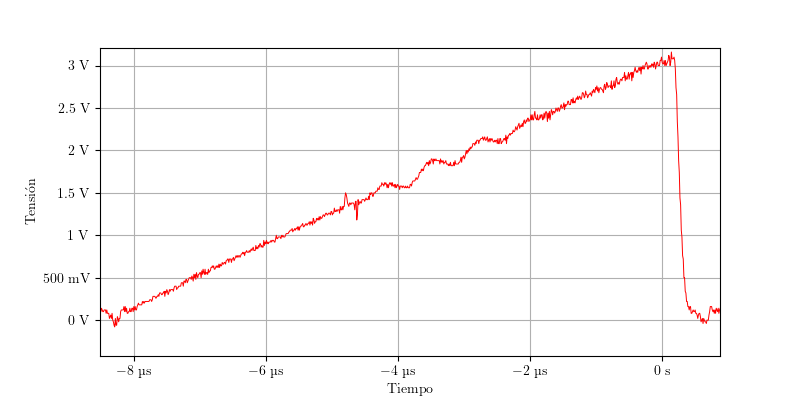
\includegraphics[width=\textwidth]{images/capturas-osciloscopio/17-11-2022/5.png}
    \caption{Tensión en el capacitor $C_t$} %COMPLETAR
    \label{fig:ct_v}
\end{figure}

% La forma de onda de Ct es la esperada, pero la de DTC?

\begin{figure}[H]
    \centering
    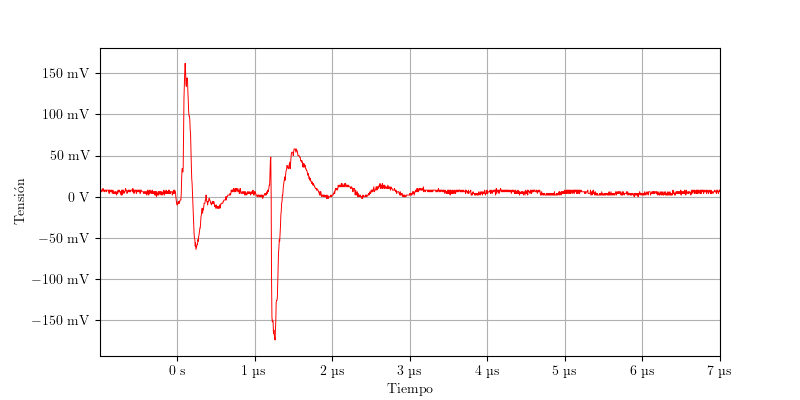
\includegraphics[width=\textwidth]{images/capturas-osciloscopio/TL494/DTC_v.png}
    \caption{Tensión a la salida del pin DTC del TL494} %COMPLETAR
    \label{fig:dtc_v}
\end{figure}

Se observa una disminución en la frecuencia de la forma de onda a aproximadamente $f=112kHz$. 
En esta señal se observa mejor la oscilación no deseada de $f_{osc}=1.25MHz$, 
la cual estará presente en muchas de las formas de onda que se analizarán a continuación. 

% 1) Señal PWM

% Se toma la salida por el colector de los transistores del circuito integrado. 
% Su forma de onda son pulsos rectangulares. 
% Amplitud: 0V a Vdrv dados por la tensión de alimentación.
% Frecuencia de 125kHz dada por el capacitor Ct=1nF y $Rt=8k\Omega$ mediante el potenciómetro. 
% Tiempo de encendido: permite controlar el ciclo de trabajo mediante un potenciómetro. 
% Esta señal se mide en 3 condiciones diferentes: 
% A) Sin el convertidor forward conectado
% B) Con el convertidor forward conectado pero sin su alimentación de 36V
% C) Con el convertidor forward conectado y alimentado

% 2) Diente de Sierra 

% Tensión en el capacitor Ct. 

% 3) Tensión en el puerto DTC 

\subsection{Etapa de ganancia de corriente}

% En las figuras \ref{fig:pwm_iout_sin_bjt} y \ref{fig:pwm_iout_con_bjt} puede observarse la corriente de salida del TL494 antes y después de agregar la etapa de ganancia de corriente, respectivamente.

% \begin{figure}[H]
%     \centering
%     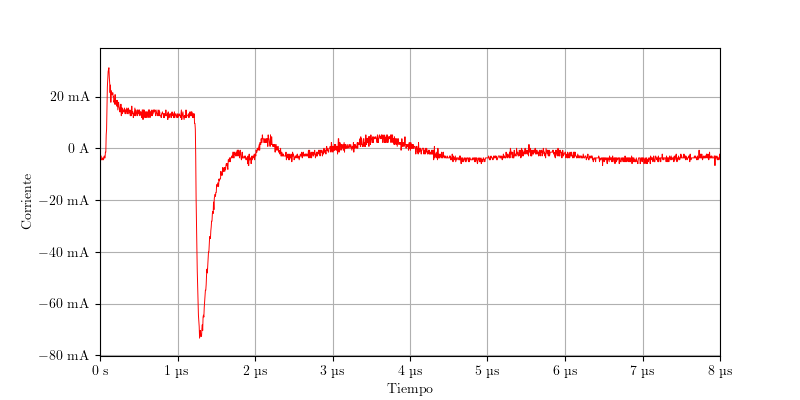
\includegraphics[width=\textwidth]{images/capturas-osciloscopio/TL494/pwm_iout_sin_bjt.png}
%     \caption{Corriente a la salida del TL494 sin colocar la etapa intermedia de ganancia de corriente}
%     \label{fig:pwm_iout_sin_bjt}
% \end{figure}

% \begin{figure}[H]
%     \centering
%     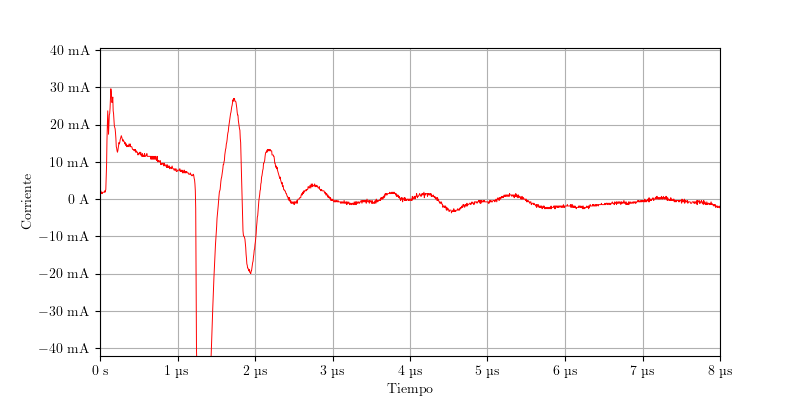
\includegraphics[width=\textwidth]{images/capturas-osciloscopio/BJT/bjt-iin-con-etapa.png}
%     \caption{Corriente a la salida del TL494 con la etapa intermedia de ganancia de corriente}
%     \label{fig:pwm_iout_con_bjt}
% \end{figure}

% Puede observarse que las oscilaciones aumentan. %WHAT?

En la figura \ref{fig:osc:3} se muestra la forma de onda de la tensión de salida de la etapa de ganancia de corriente.
Esta debería ser una señal PWM con un período de $8\mu s$ y un ancho de pulso de aproximadamente 40\%.

% Dado que la etapa posee ganancia de tensión unitaria, su forma de onda es aproximadamente igual a la tensión de salida del TL494. 
% Las oscilaciones fueron eliminadas mediante la red snubber. 

\begin{figure}[H]
    \centering
    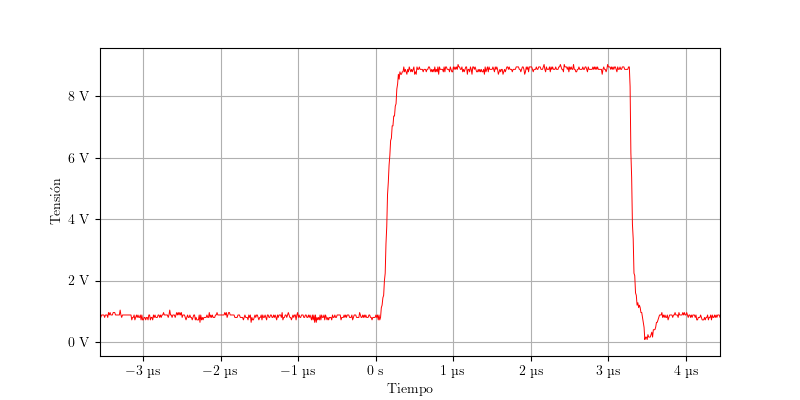
\includegraphics[width=0.8\textwidth]{images/capturas-osciloscopio/17-11-2022/3.png}
    \caption{Tensión a la salida de la etapa de ganancia de corriente}
    \label{fig:osc:3}
\end{figure}

\begin{figure}[H]
    \centering
    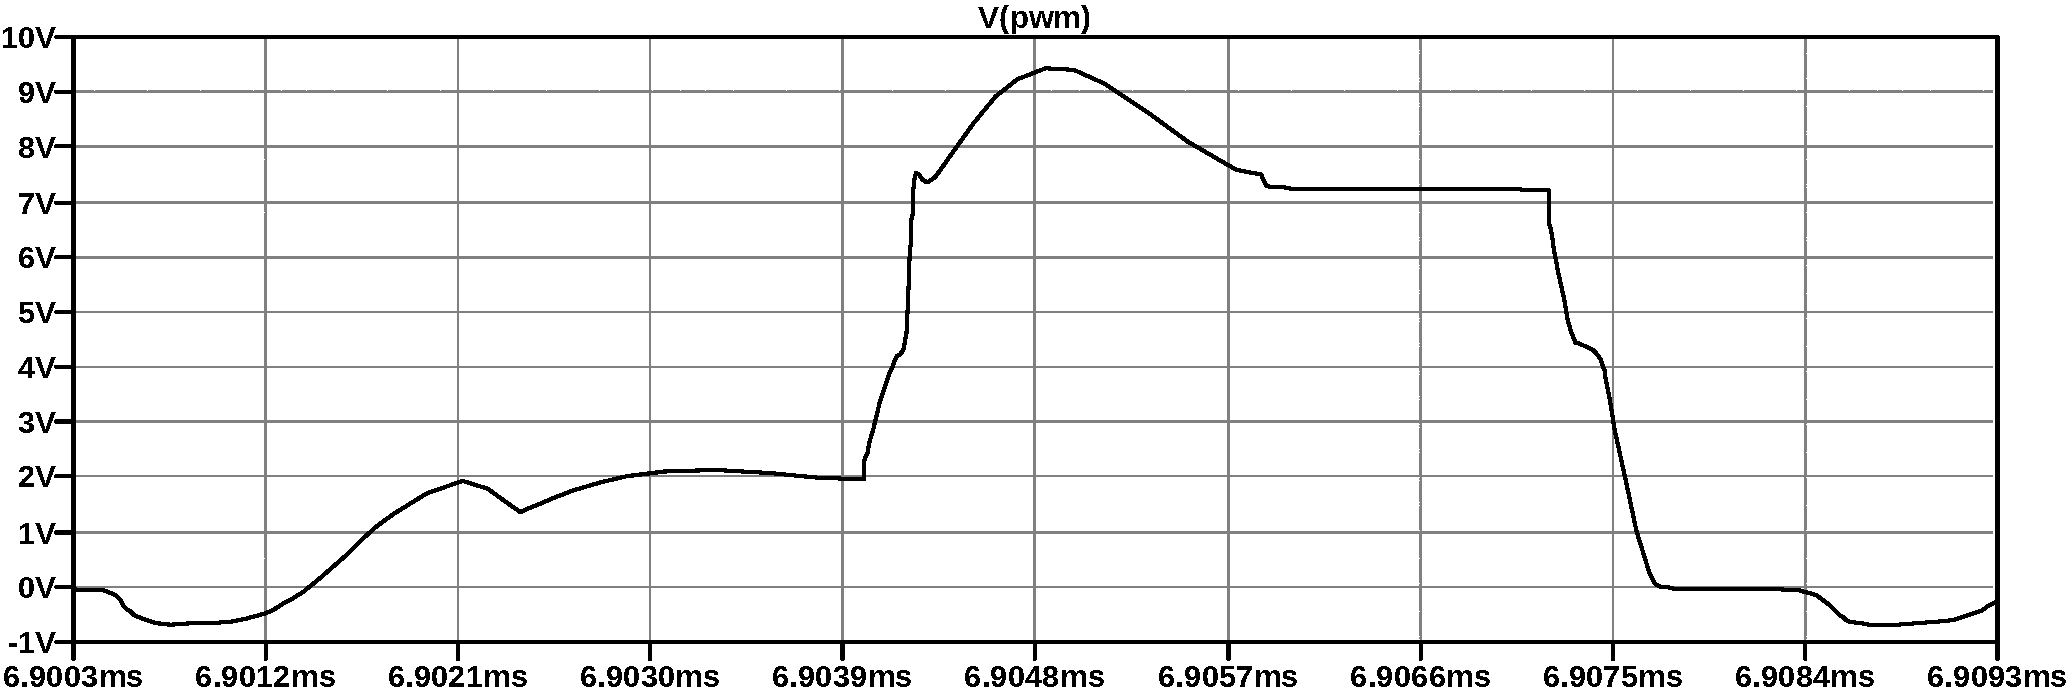
\includegraphics[width=\textwidth]{images/sim/3.pdf}
    \caption{Simulación de la tensión a la salida de la etapa de ganancia de corriente}
    \label{fig:sim:3}
\end{figure}

Se observa una mejora considerable en la forma de onda de la señal, incluso dando mejores resultados que el simulador. %Porque estamos re masa.

La función más importante de esta etapa es la de mejorar la forma de onda de la señal PWM, que al comparar las figuras \ref{fig:osc_pwm_vout_disconnected} y \ref{fig:pwm_vout_sin_bjt} se puede observar que se ha mejorado considerablemente.

\begin{figure}[H]
    \centering
    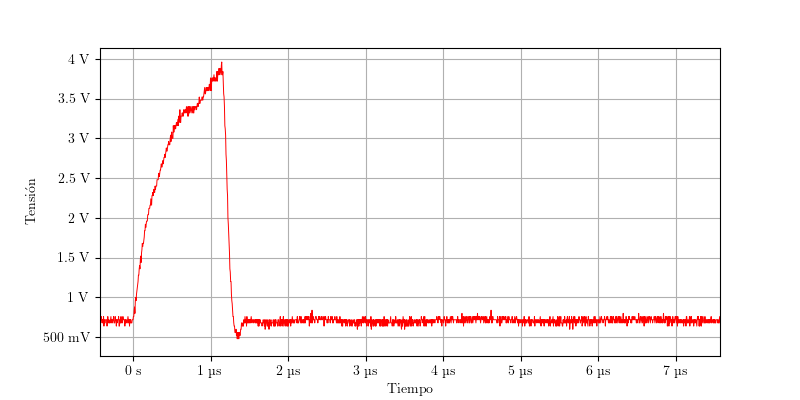
\includegraphics[width=\textwidth]{images/capturas-osciloscopio/TL494/pwm_vout_sin_bjt.png}
    \caption{Tensión a la salida del TL494 sin colocar la etapa intermedia de ganancia de corriente}
    \label{fig:pwm_vout_sin_bjt}
\end{figure}

% 1) Corriente sin la etapa 
% DONE

% 2) Corriente de entrada y de salida con la etapa

% 3) Tensión a la salida sin la etapa
% DONE

% 3) Tensión a la salida con la etapa
% DONE

% Hay que ver eso de las oscilaciones en la corriente

\subsection{Driver}

En la figura \ref{fig:driver_vout_connected} se muestra la tensión de salida del driver, que coincide con la tensión entre \textit{gate} y \textit{source} del MOSFET de lado alto.
Se puede ver que también están presentes las oscilaciones de alta frecuencia que se observan en la salida del TL494.

\begin{figure}[H]
    \centering
    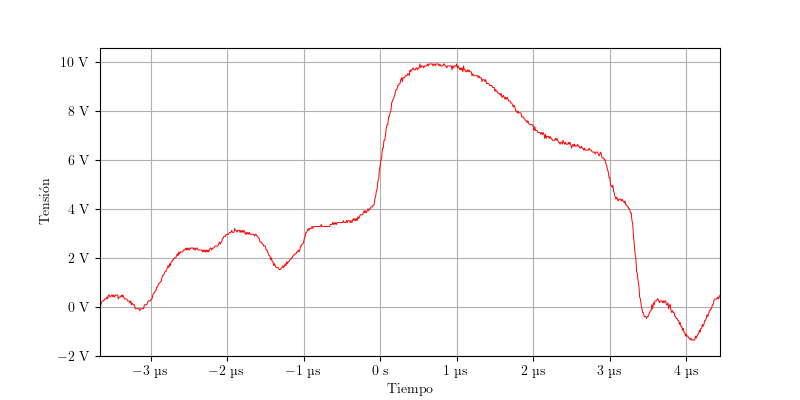
\includegraphics[width=\textwidth]{images/capturas-osciloscopio/17-11-2022/31.png} %Acá tuve que dejar la simulación vieja, porque la nueva está desfasada y esta hecha con otro D, queda mal
    \caption{Tensión a la salida del driver}
    \label{fig:driver_vout_connected}
\end{figure}

En la figura \ref{fig:sim:driver_vout_connected} puede verse los resultados de la simulación.

\begin{figure}[H]
    \centering
    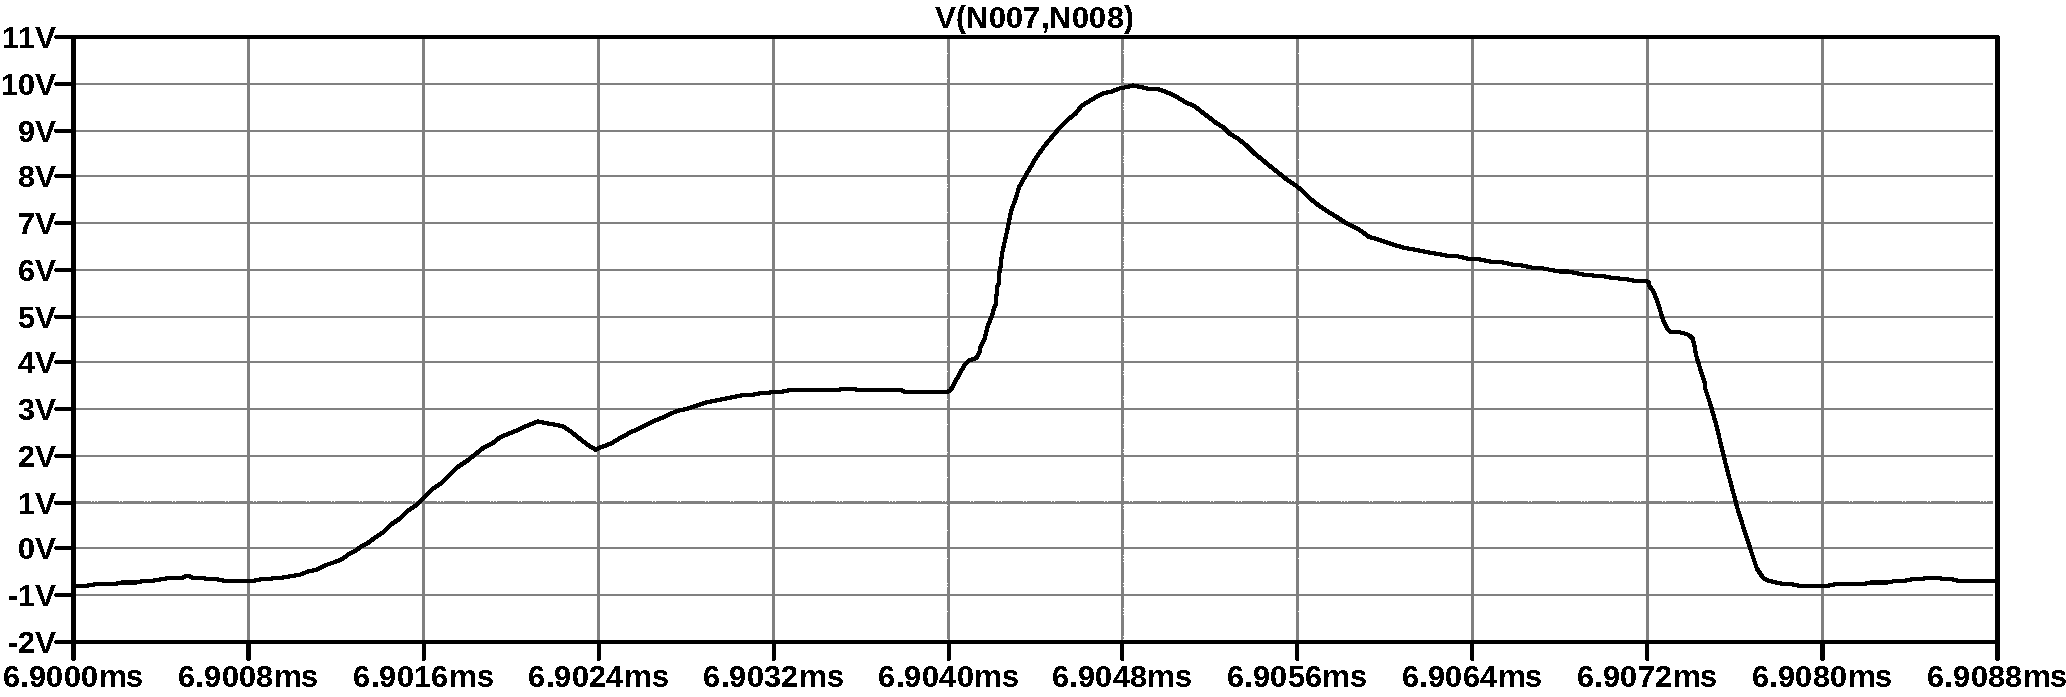
\includegraphics[width=\textwidth]{images/sim/15.pdf}
    \caption{Simulación de la tensión a la salida del driver}
    \label{fig:sim:driver_vout_connected}
\end{figure}
% HAY QUE ORDENAR ESTAS 2

En la figura \ref{fig:driver_expected_waveforms} se muestran algunas formas de onda del circuito del driver con las que se hicieron comparaciones para verificar su correcto funcionamiento.

\begin{figure}[H]
    \centering
    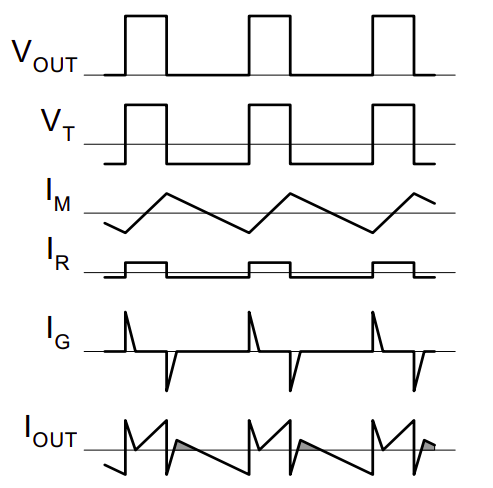
\includegraphics[width=0.7\textwidth]{images/driver_expected_waveforms.png}
    \caption{Formas de onda esperadas de distintas señales del driver \cite{gatedrivers}}
    \label{fig:driver_expected_waveforms}
\end{figure}

A continuación se presentan formas de ondas variadas del driver, comparándolas con las simulaciones para verificar su funcionamiento.
% 1) Tensiones en el transformador de señal 

    % Forma de onda: Rectangular 
    % Amplitud: -Vc a Vdrv-Vc 
    % Son iguales dada la relación 1:1 del transformador. 

\begin{figure}[H]
    \centering
    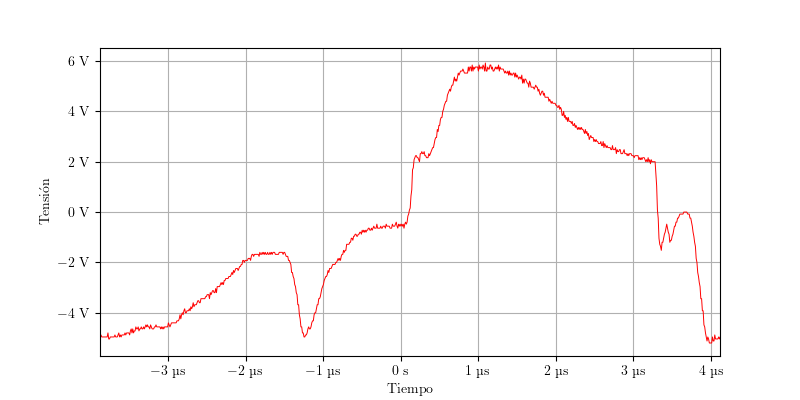
\includegraphics[width=0.9\textwidth]{images/capturas-osciloscopio/17-11-2022/7.png}
    \caption{Tensión en el primario del transformador del driver}
    \label{fig:osc:7}
\end{figure}

\begin{figure}[H]
    \centering
    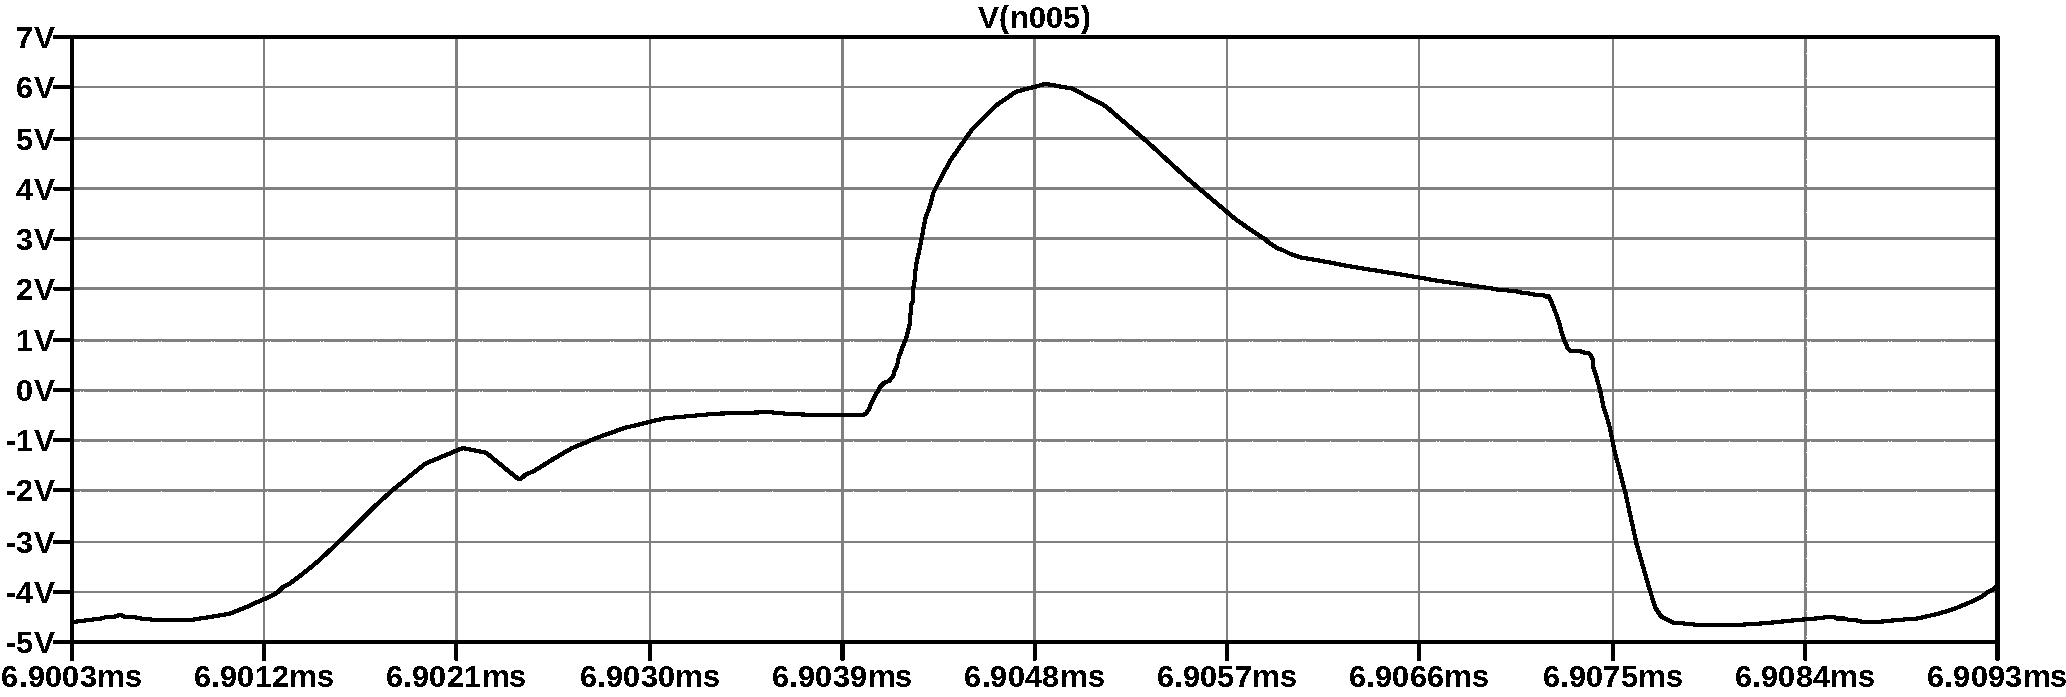
\includegraphics[width=\textwidth]{images/sim/4.pdf}
    \caption{Simulación de la tensión en el primario del transformador del driver}
    \label{fig:sim:4}
\end{figure}

La amplitud y la forma de onda de la señal del prototipo coinciden respecto a la simulación. 
Se observan unos picos en los flancos de subida y de bajada. 

\begin{figure}[H]
    \centering
    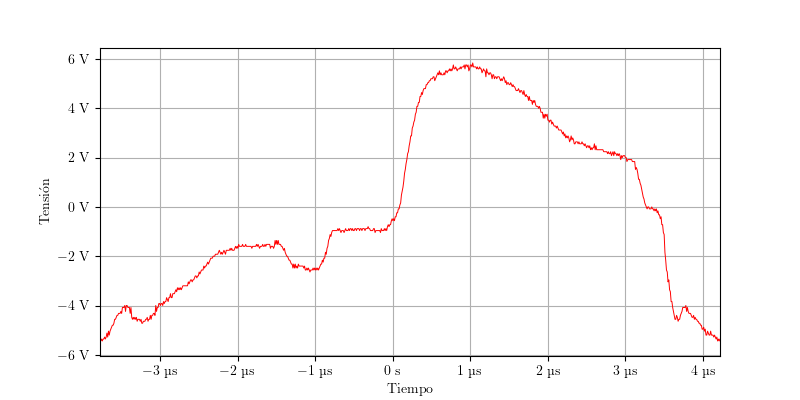
\includegraphics[width=0.9\textwidth]{images/capturas-osciloscopio/17-11-2022/9.png}
    \caption{Tensión en el secundario del transformador del driver}
    \label{fig:osc:9}
\end{figure}

\begin{figure}[H]
    \centering
    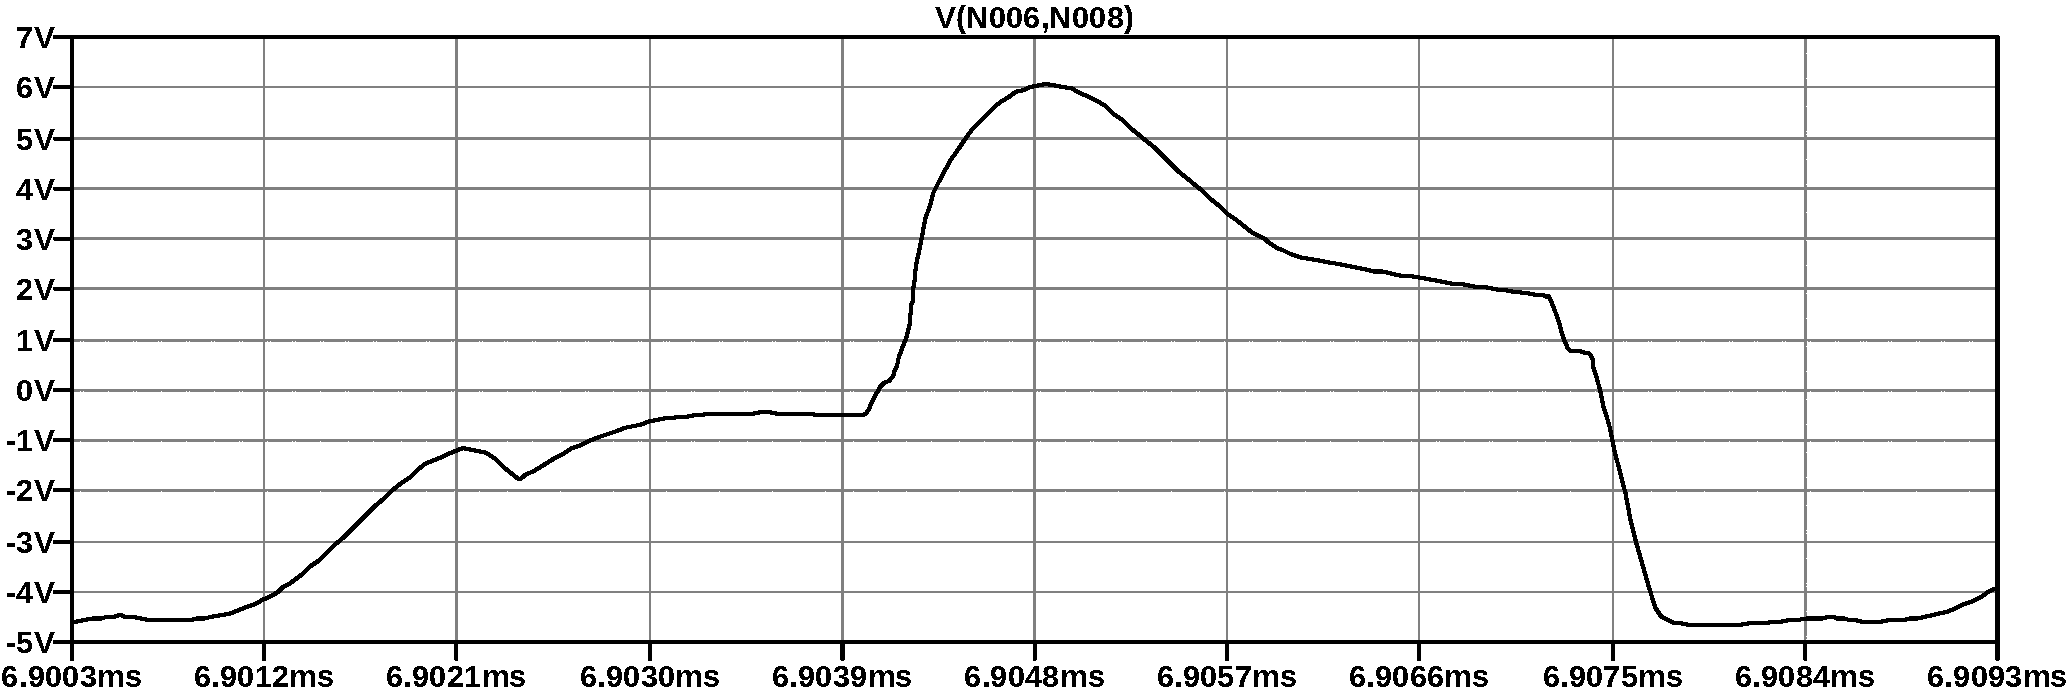
\includegraphics[width=\textwidth]{images/sim/5.pdf}
    \caption{Simulación de la tensión en el secundario del transformador del driver}
    \label{fig:sim:5}
\end{figure}

Para el caso del secundario, las formas de onda también coinciden. 
Se observa un pico solo en el flanco de bajada.

En las figuras \ref{fig:osc:11} y \ref{fig:sim:6} se muestran la forma de onda de la corriente por el primario del transformador del driver junto con su simulación.

\begin{figure}[H]
    \centering
    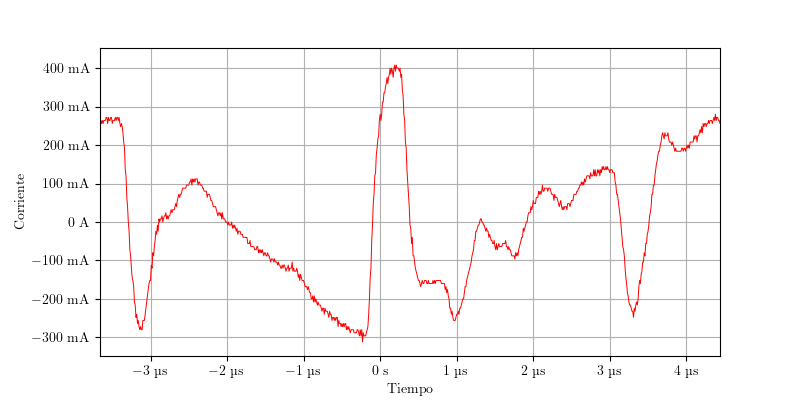
\includegraphics[width=\textwidth]{images/capturas-osciloscopio/17-11-2022/11.png}
    \caption{Corriente por el primario del transformador del driver}
    \label{fig:osc:11}
\end{figure}

\begin{figure}[H]
    \centering
    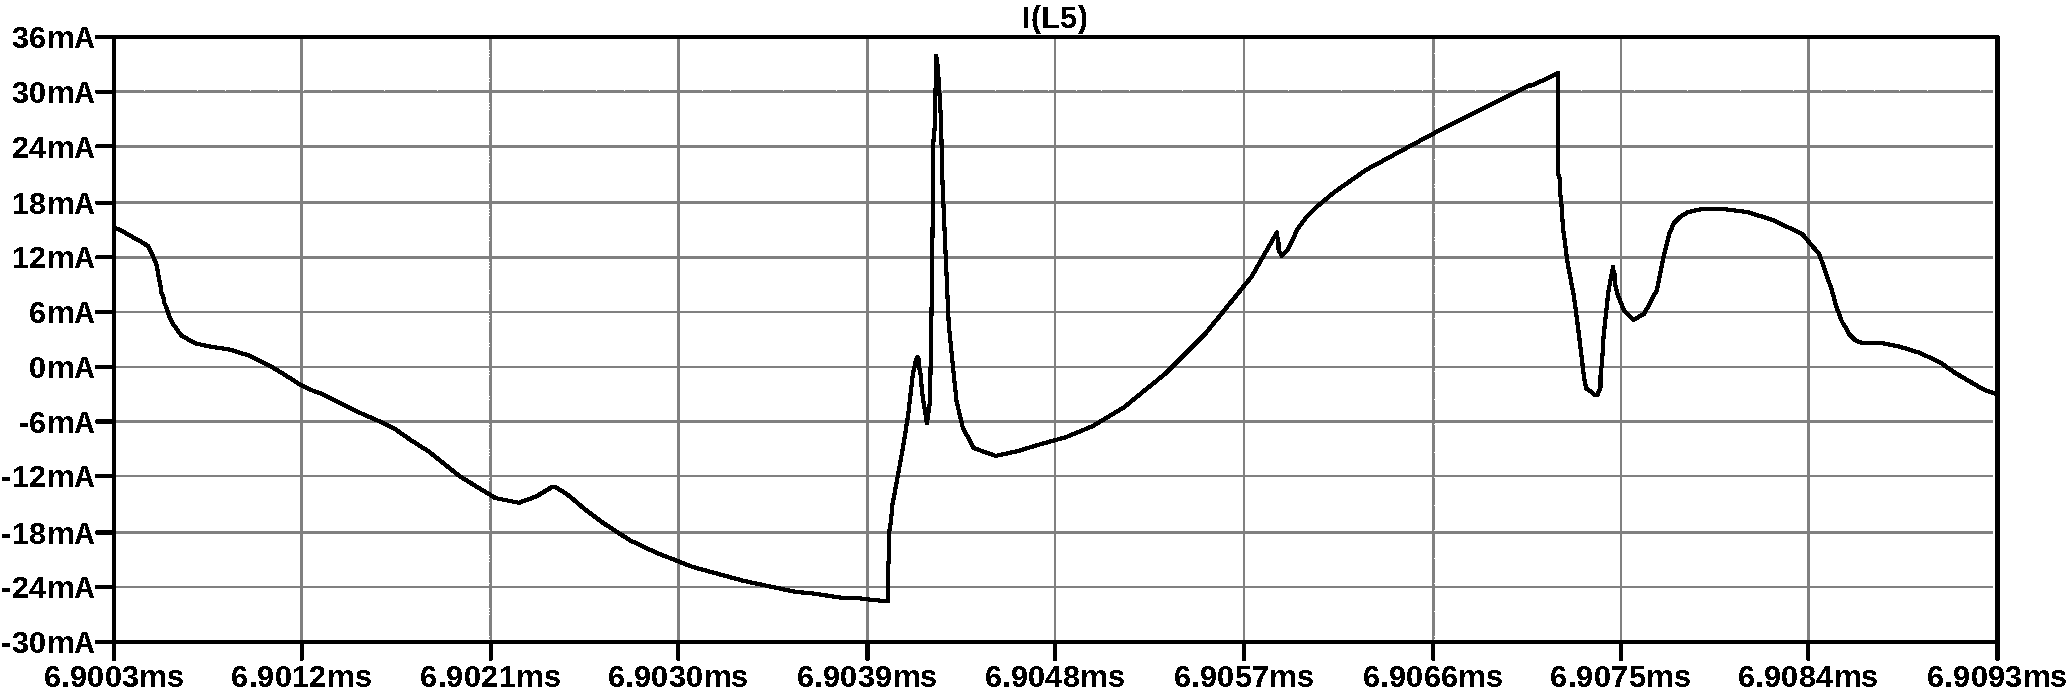
\includegraphics[width=\textwidth]{images/sim/6.pdf}
    \caption{Simulación de la corriente por el primario del transformador del driver}
    \label{fig:sim:6}
\end{figure}

La forma de onda del prototipo presenta una deformación y posee levemente mayor amplitud. 

\begin{figure}[H]
    \centering
    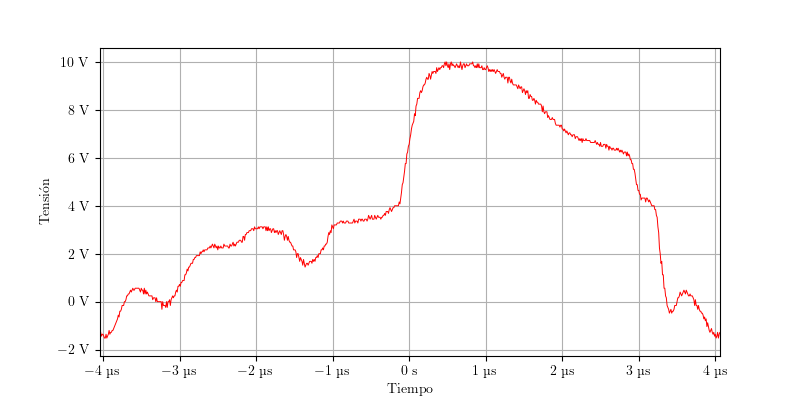
\includegraphics[width=\textwidth]{images/capturas-osciloscopio/17-11-2022/13.png}
    \caption{Corriente por la resistencia entre \textit{gate} y \textit{source} del MOSFET de lado alto}
    \label{fig:osc:13}
\end{figure}

\begin{figure}[H]
    \centering
    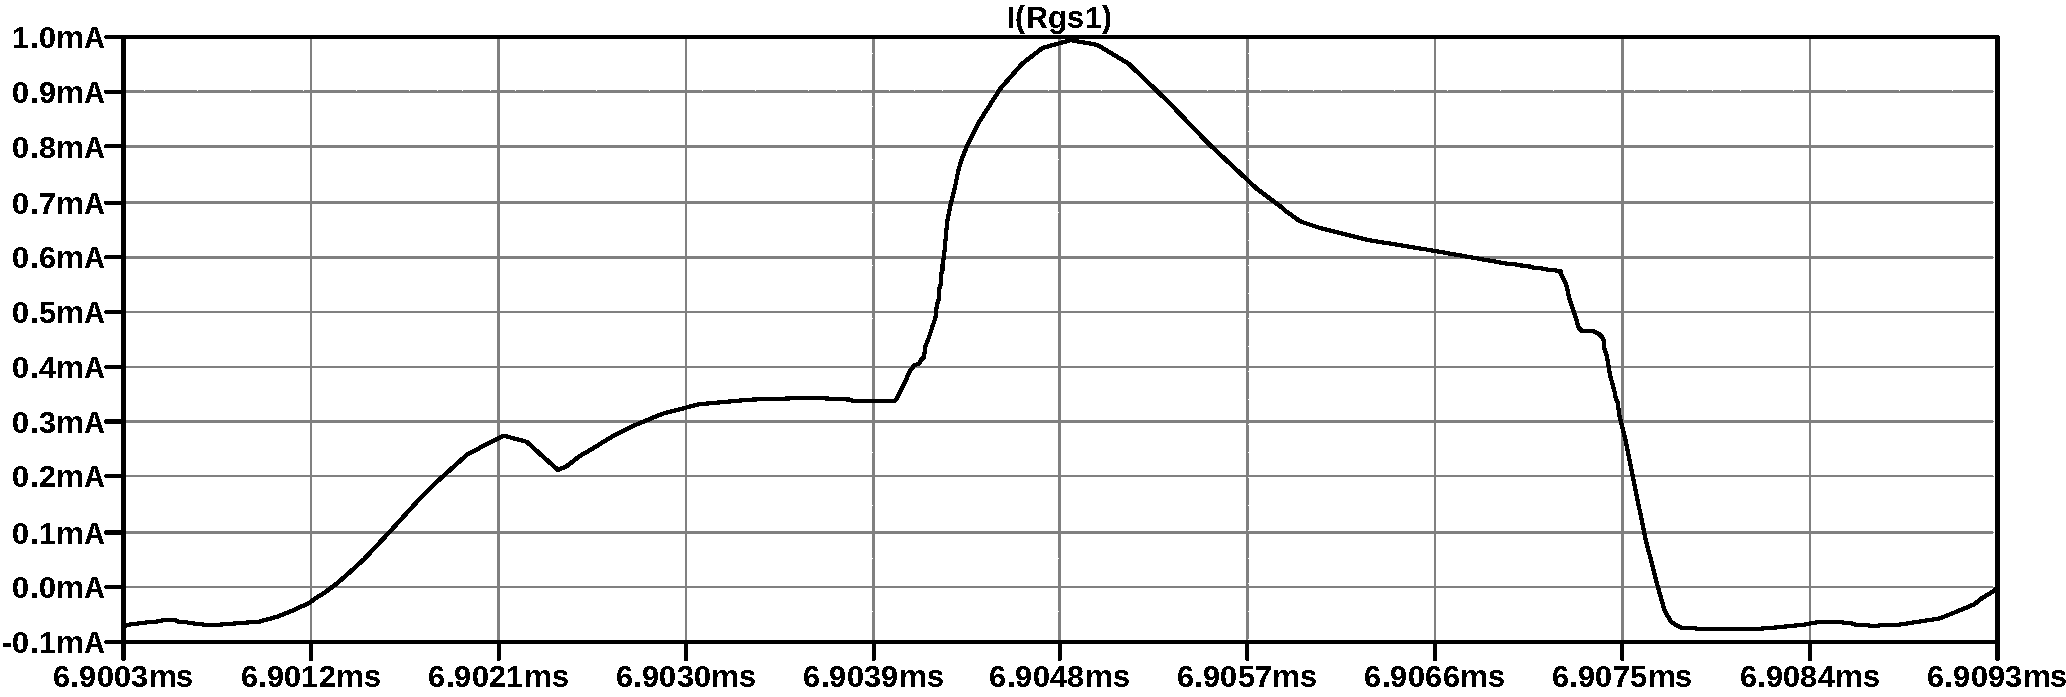
\includegraphics[width=\textwidth]{images/sim/7.pdf}
    \caption{Simulación de la corriente por la resistencia $R_{gs}$}
    \label{fig:sim:7}
\end{figure}

La amplitud y la forma de onda de la señal del prototipo coinciden respecto a la simulación. 
Presenta la oscilación de $f_{osc}=1.25MHz$. 

% 2) Tensión Gate del MOSFET high side % Sería vout del driver?
% DONE

    % Forma de onda: Rectangular 
    % Amplitud: -Vd a Vdrv-Vd
    % Vd: Tensión en el diodo del secundario

% 3) Corriente de salida % FALTA MEDIR LAS CORRIENTES CON LA PCB

    % Compuesta por:

    % A) Corriente magnetizante

        % Forma de onda: triangular
        % Se mide en la Rc del primario. 

    % B) Corriente por Rgs

        % Forma de onda: rectangular

    % C) Corriente por Gate

        % Forma de onda: diente de sierra invertida y espejada con tiempo muerto 

\subsection{Convertidor}

% Agregar intro
\subsubsection{MOSFETs}

% 1) Vgs de ambos MOSFETs %Ya se midió en otros lados

% 2) Vds de ambos MOSFETs

En las figuras \ref{fig:vds_high} y \ref{fig:vds_low} se muestran las tensiones en los terminales \textit{drain} y \textit{source} de los MOSFETs del convertidor forward doble switch.
Para comparar, se muestra en las figuras \ref{fig:vds_simulation_high} y \ref{fig:vds_simulation_low} las tensiones $V_{DS}$ de los MOSFETs simulados en LTSpice. 

\begin{figure}[H]
    \centering
    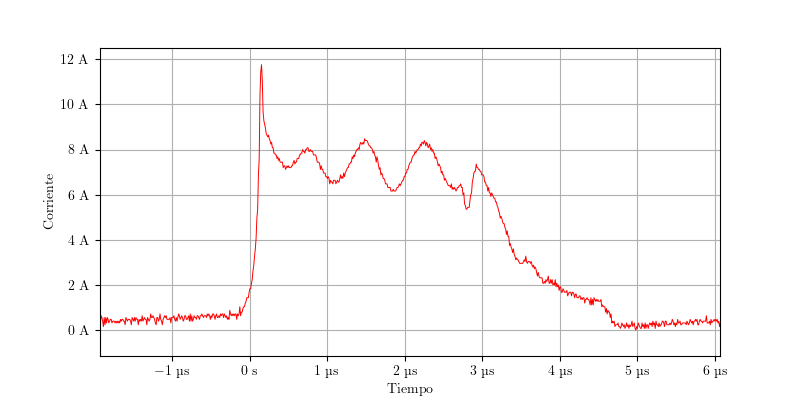
\includegraphics[width=0.9\textwidth]{images/capturas-osciloscopio/17-11-2022/33.png}
    \caption{Tensión $V_{DS}$ en el MOSFET de lado alto}
    \label{fig:vds_high}
\end{figure}

\begin{figure}[H]
    \centering
    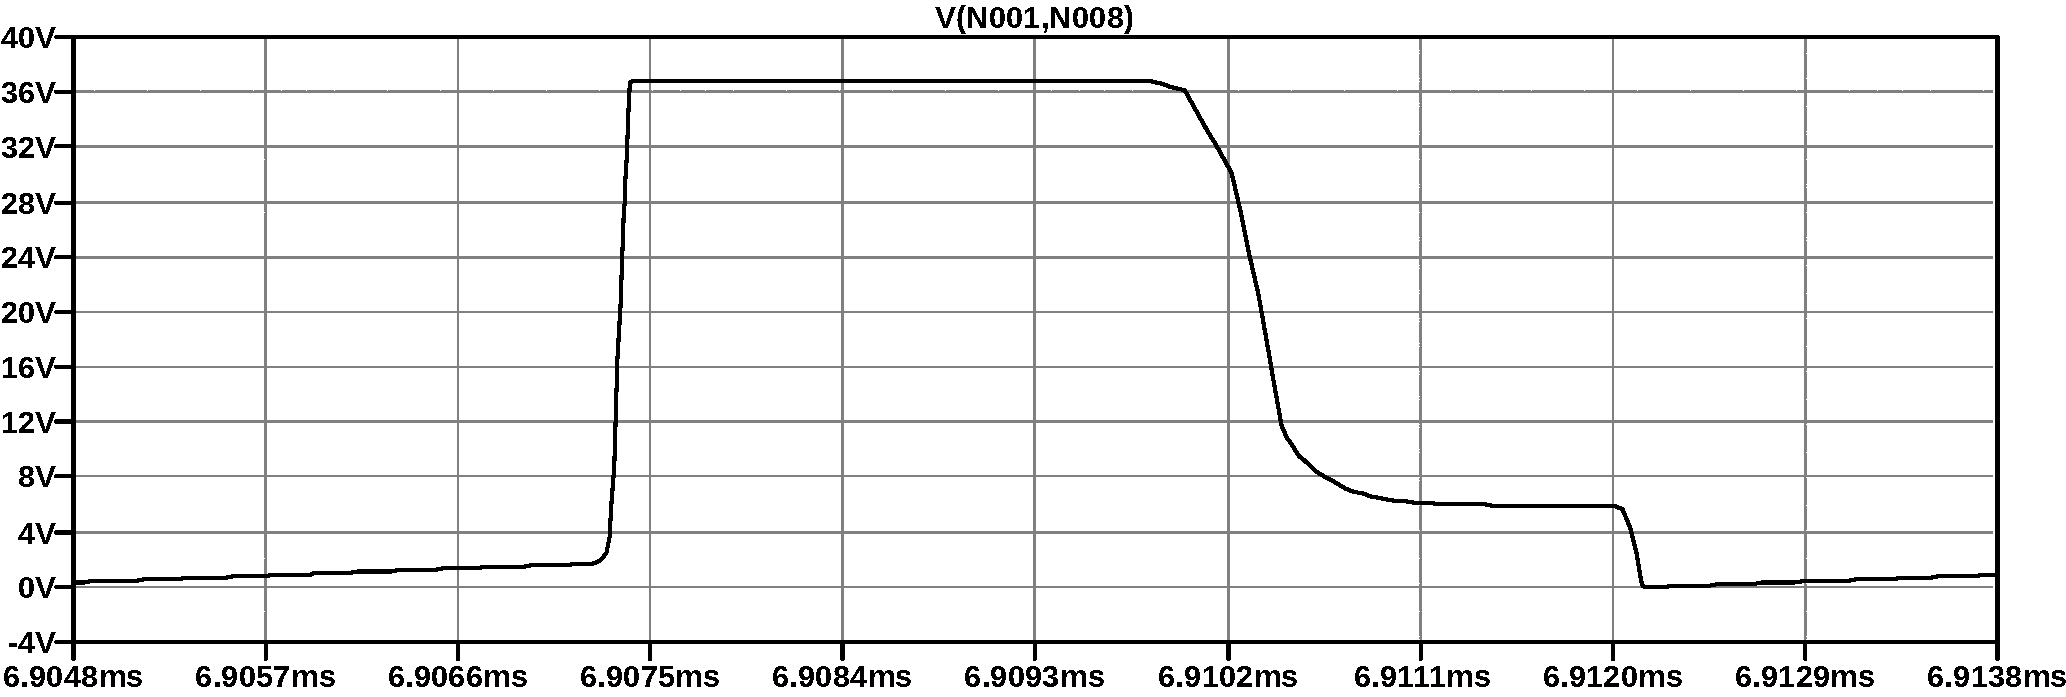
\includegraphics[width=\textwidth]{images/sim/16.pdf}
    \caption{Tensión $V_{DS}$ en el MOSFET de lado alto simulado en LTspice}
    \label{fig:vds_simulation_high}
\end{figure}

\begin{figure}[H]
    \centering
    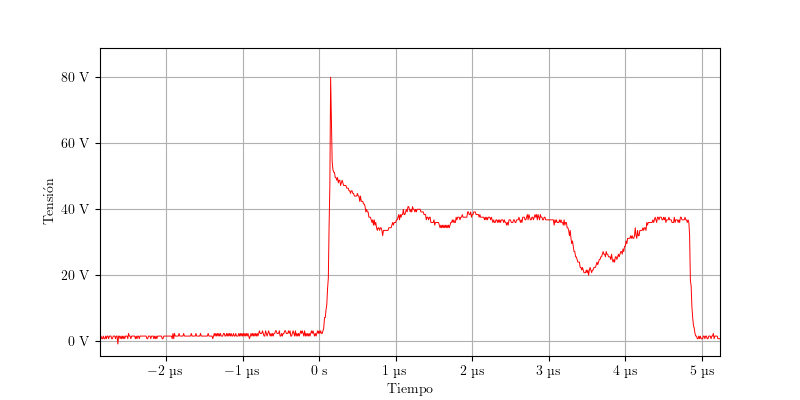
\includegraphics[width=0.9\textwidth]{images/capturas-osciloscopio/17-11-2022/36.png}
    \caption{Tensión $V_{DS}$ en el MOSFET de lado bajo}
    \label{fig:vds_low}
\end{figure}

\begin{figure}[H]
    \centering
    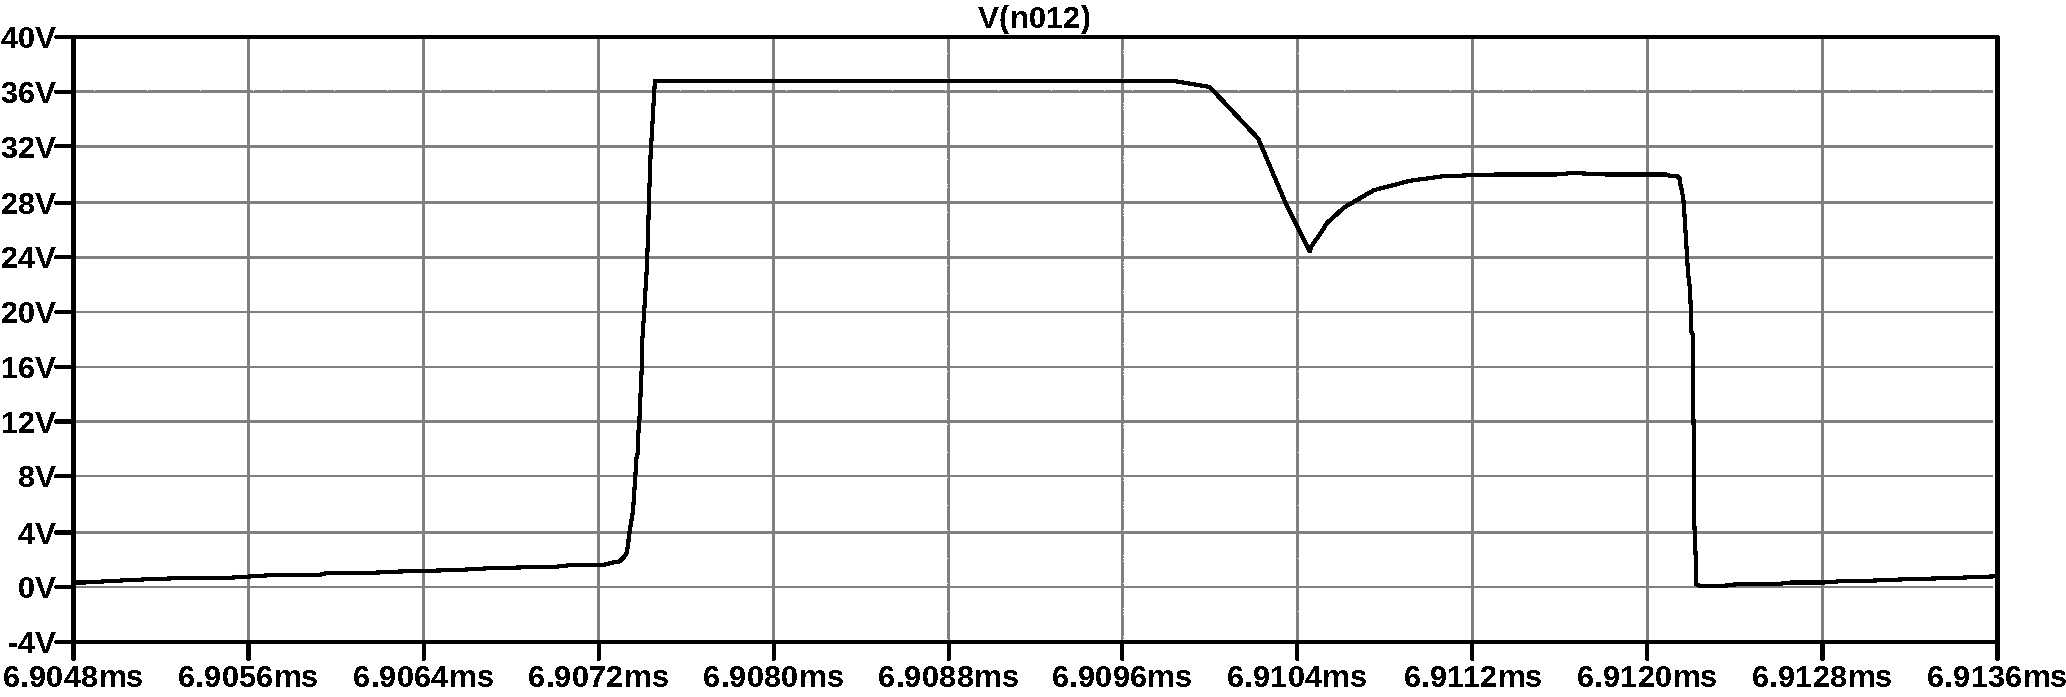
\includegraphics[width=\textwidth]{images/sim/18.pdf}
    \caption{Tensión $V_{DS}$ en el MOSFET de lado bajo side simulado en LTspice}
    \label{fig:vds_simulation_low}
\end{figure}

% 3) Idrain de ambos MOSFETs

En las figuras \ref{fig:osc:20} y \ref{fig:osc:22} puede verse la corriente por el terminal \textit{drain} de los MOSFETs del convertidor. Las figuras \ref{fig:sim:10} y \ref{fig:sim:11} muestran sus simulaciones, respectivamente.

\begin{figure}[H]
    \centering
    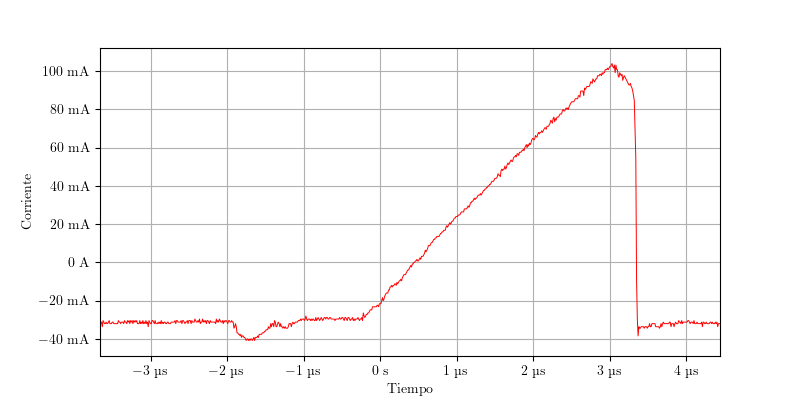
\includegraphics[width=0.8\textwidth]{images/capturas-osciloscopio/17-11-2022/20.png}
    \caption{Corriente que circula por el \textit{drain} del MOSFET de lado alto}
    \label{fig:osc:20}
\end{figure}

\begin{figure}[H]
    \centering
    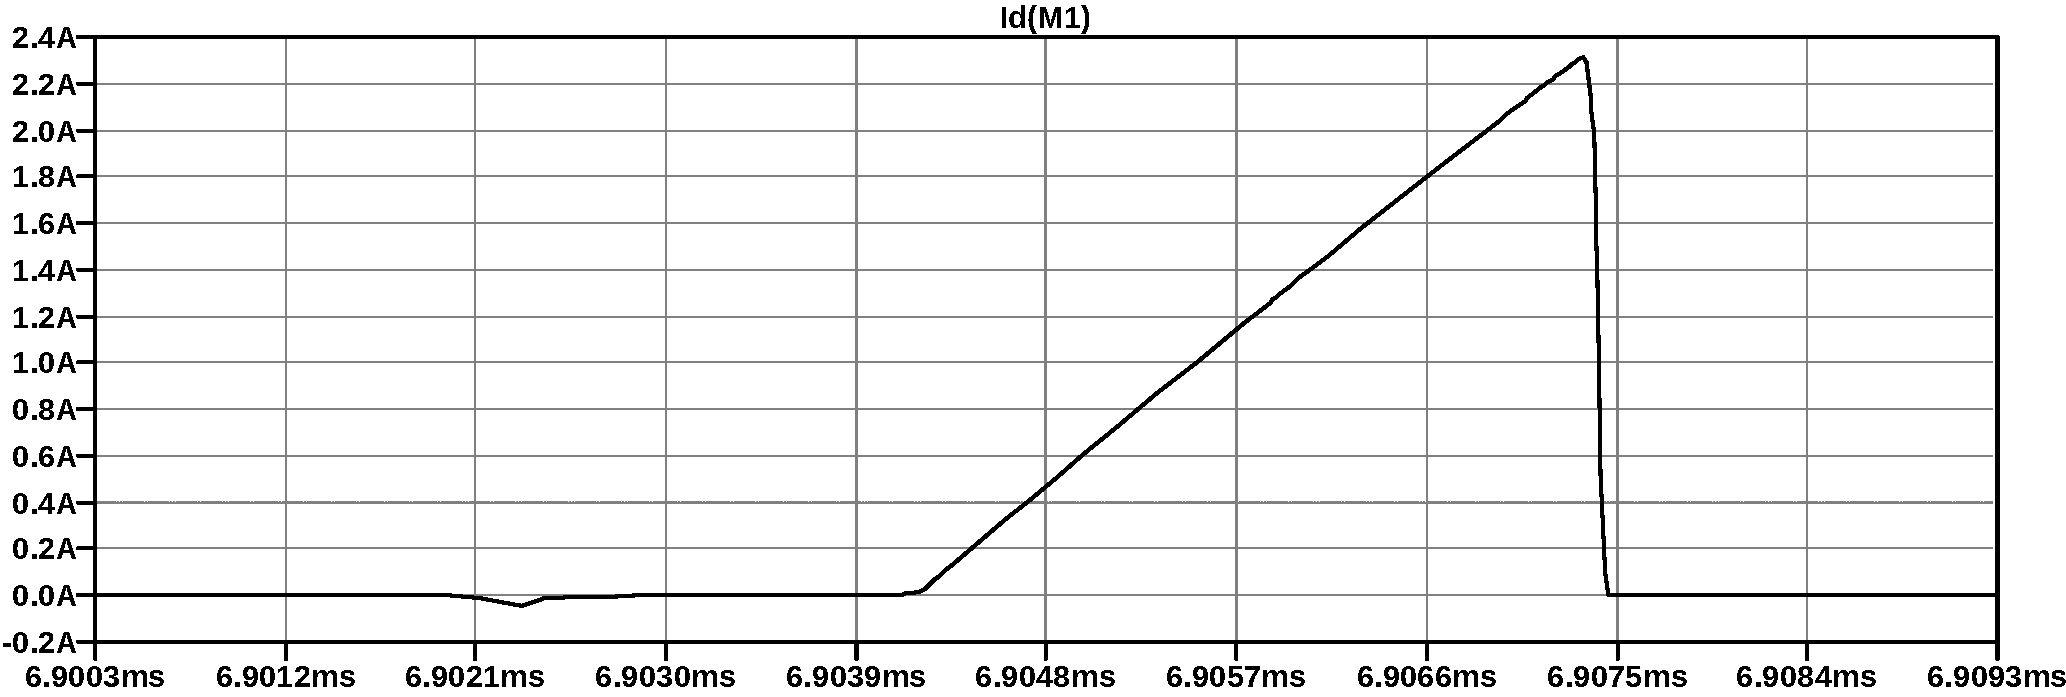
\includegraphics[width=\textwidth]{images/sim/10.pdf}
    \caption{Simulación de la corriente que circula por el \textit{drain} del MOSFET de lado alto}
    \label{fig:sim:10}
\end{figure} 

\begin{figure}[H]
    \centering
    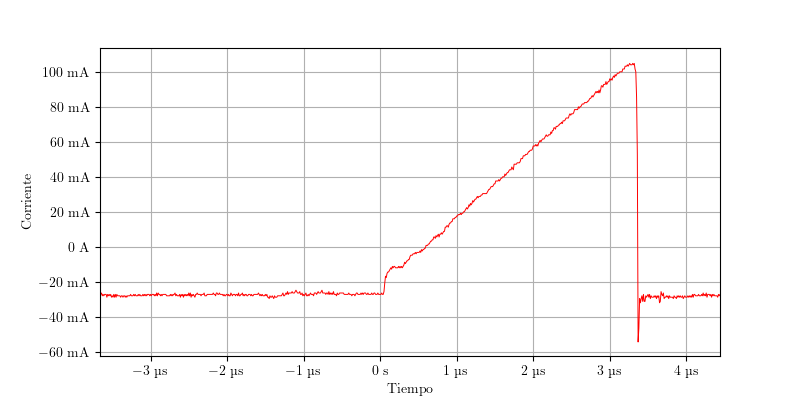
\includegraphics[width=0.8\textwidth]{images/capturas-osciloscopio/17-11-2022/22.png}
    \caption{Corriente que circula por el \textit{drain} del MOSFET de lado bajo}
    \label{fig:osc:22}
\end{figure}

\begin{figure}[H]
    \centering
    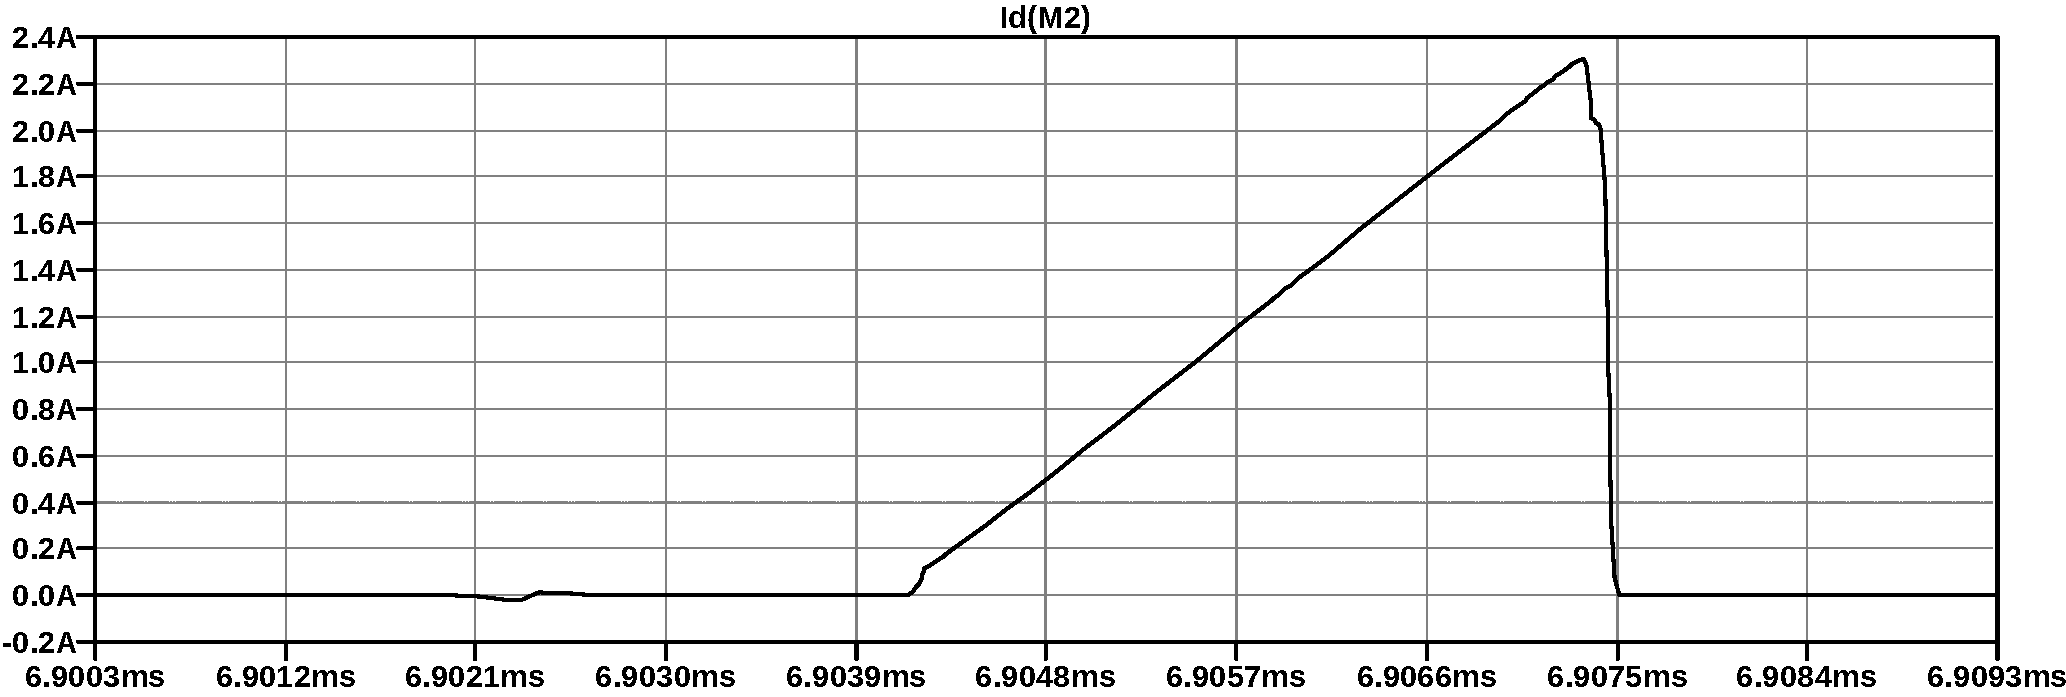
\includegraphics[width=\textwidth]{images/sim/11.pdf}
    \caption{Simulación de la corriente que circula por el \textit{drain} del MOSFET de lado bajo}
    \label{fig:sim:11}
\end{figure}

El prototipo presenta un sobrepico negativo en el flanco de bajada del MOSFET de lado bajo. 
También se observa que la amplitud de la señal simulada es mucho mayor.

Como último punto de los MOSFETs, se muestran en las figuras \ref{fig:osc:15} y \ref{fig:osc:17} las corrientes por \textit{gate} del MOSFET de lado alto y bajo, respectivamente.
Sus simulaciones pueden verse en las figuras \ref{fig:sim:8} y \ref{fig:sim:9}

\begin{figure}[H]
    \centering
    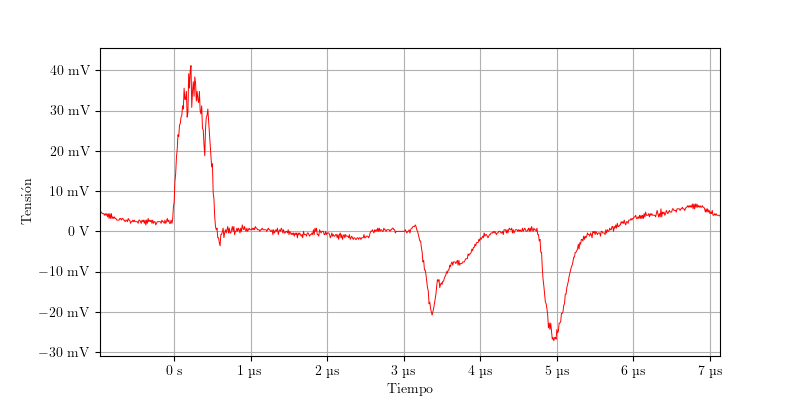
\includegraphics[width=0.8\textwidth]{images/capturas-osciloscopio/17-11-2022/15.png}
    \caption{Corriente que circula por el gate del MOSFET de lado alto}
    \label{fig:osc:15}
\end{figure}
 
\begin{figure}[H]
    \centering
    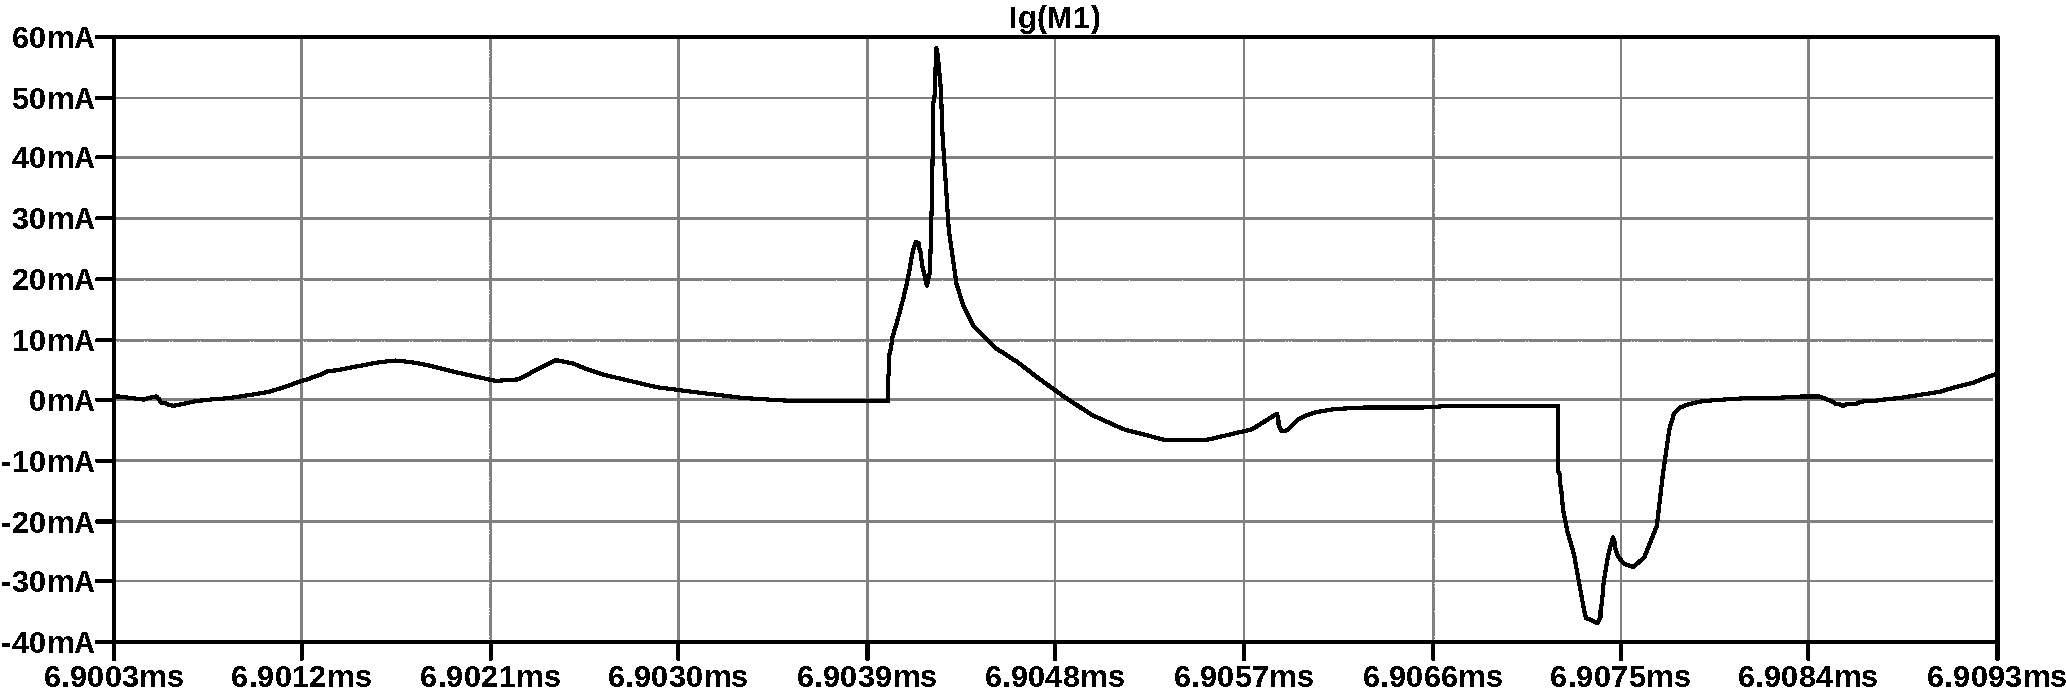
\includegraphics[width=\textwidth]{images/sim/8.pdf}
    \caption{Simulación de la crriente que circula por el gate del MOSFET de lado alto}
    \label{fig:sim:8}
\end{figure}
 
\begin{figure}[H]
    \centering
    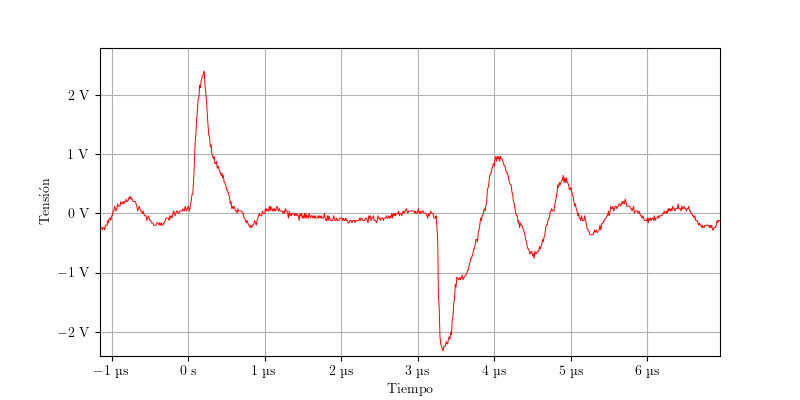
\includegraphics[width=0.8\textwidth]{images/capturas-osciloscopio/17-11-2022/17.png}
    \caption{Corriente que circula por el gate del MOSFET lado bajo}
    \label{fig:osc:17}
\end{figure}

\begin{figure}[H]
    \centering
    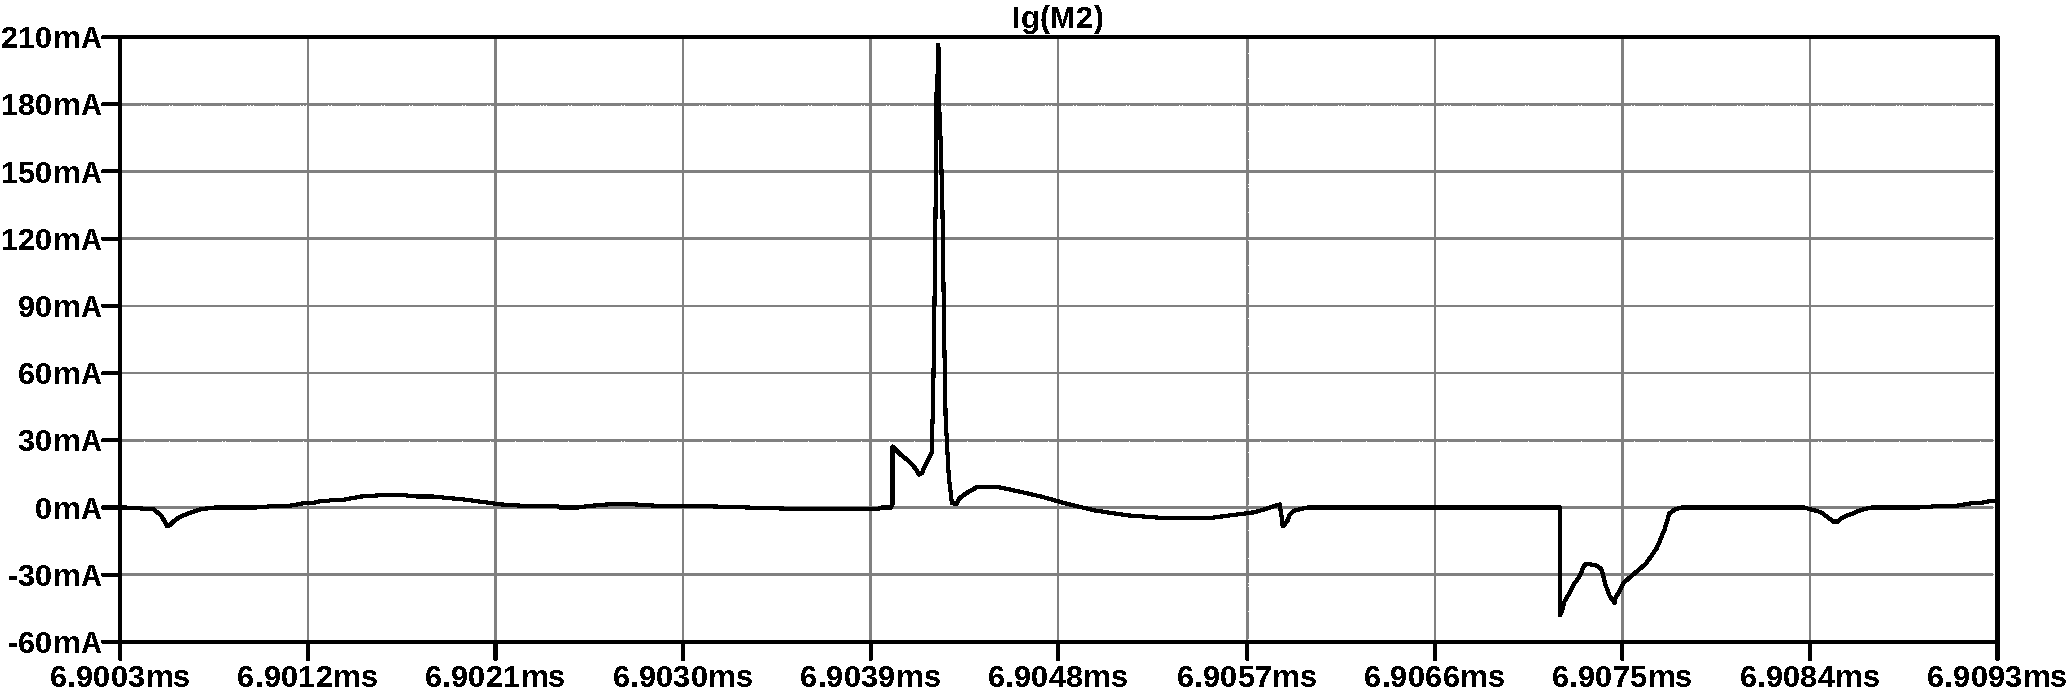
\includegraphics[width=\textwidth]{images/sim/9.pdf}
    \caption{Simulación de la crriente que circula por el gate del MOSFET de lado bajo}
    \label{fig:sim:9}
\end{figure}

\subsubsection{Transformador de potencia}
% 4) Tensiones en el E70

Las figuras \ref{fig:osc:38} y \ref{fig:osc:40} muestran las tensiones en el primario y el secundario del transformador de potencia, respectivamente. Puede observarse comparando con sus simulaciones (Figuras \ref{fig:sim:19} y \ref{fig:sim:20}) que las oscilaciones son mucho mayores en el secundario del transformador.

\begin{figure}[H]
    \centering
    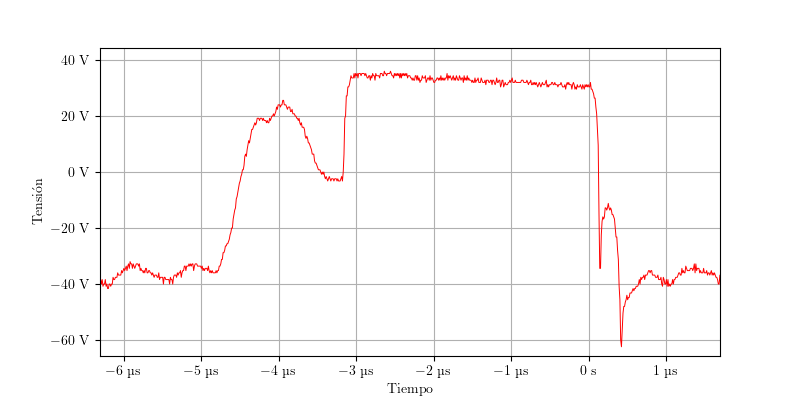
\includegraphics[width=0.8\textwidth]{images/capturas-osciloscopio/17-11-2022/38.png}
    \caption{Tensión en el primario del transformador de potencia}
    \label{fig:osc:38}
\end{figure}

\begin{figure}[H]
    \centering
    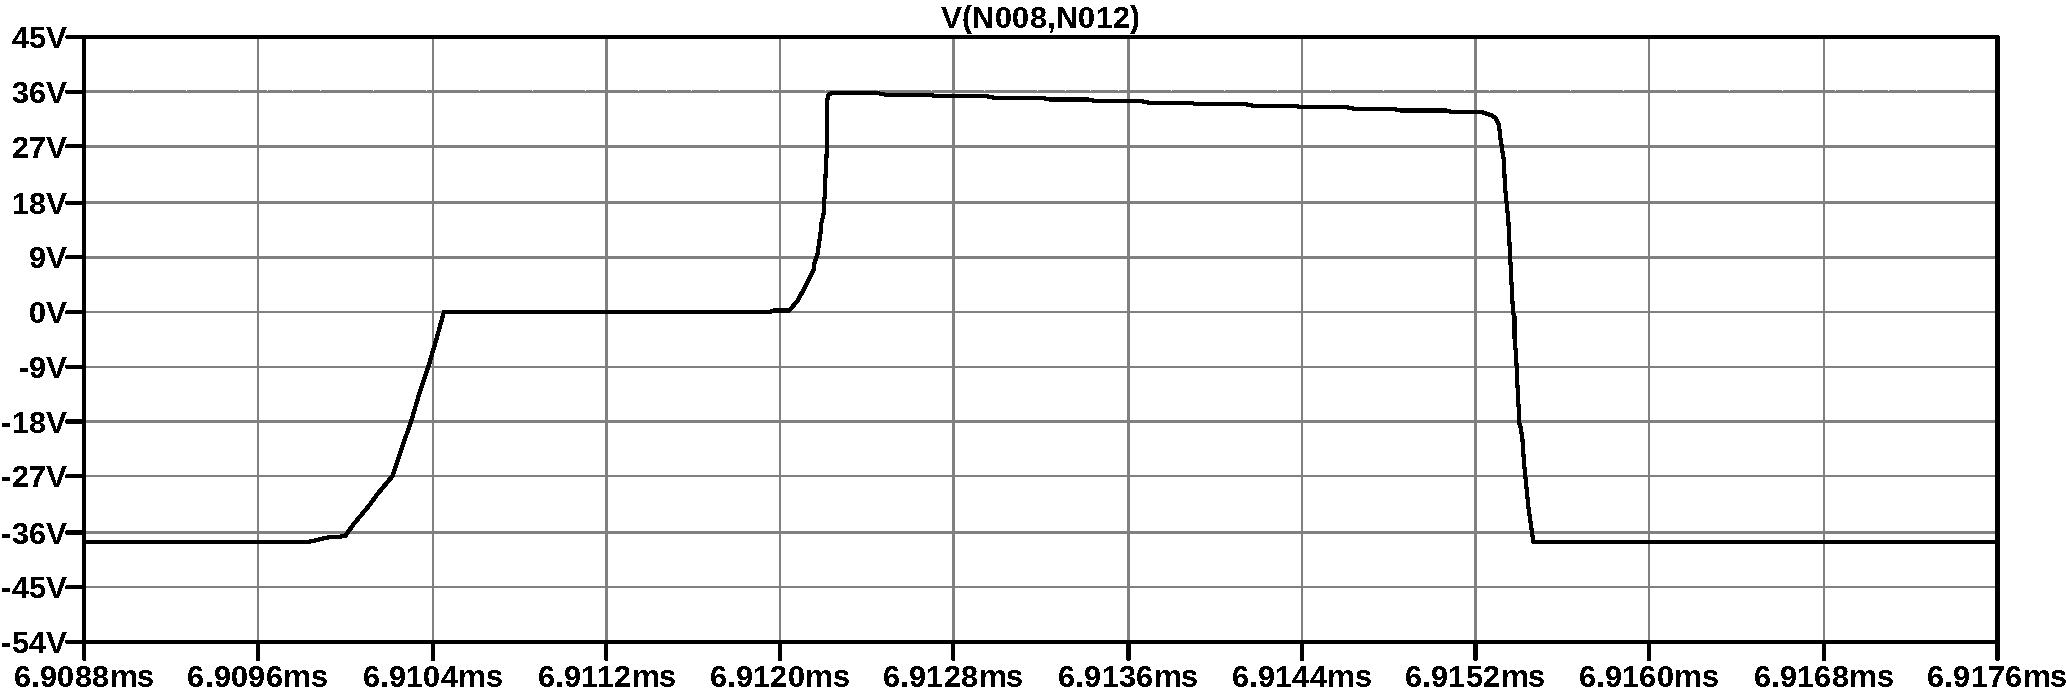
\includegraphics[width=\textwidth]{images/sim/19.pdf}
    \caption{Simulación de la tensión en el primario del transformador de potencia}
    \label{fig:sim:19}
\end{figure}

\begin{figure}[H]
    \centering
    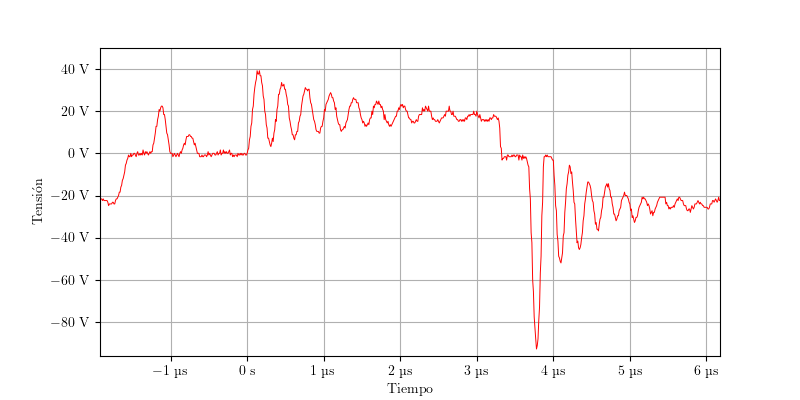
\includegraphics[width=0.8\textwidth]{images/capturas-osciloscopio/17-11-2022/40.png}
    \caption{Tensión en el secundario del transformador de potencia}
    \label{fig:osc:40}
\end{figure}

\begin{figure}[H]
    \centering
    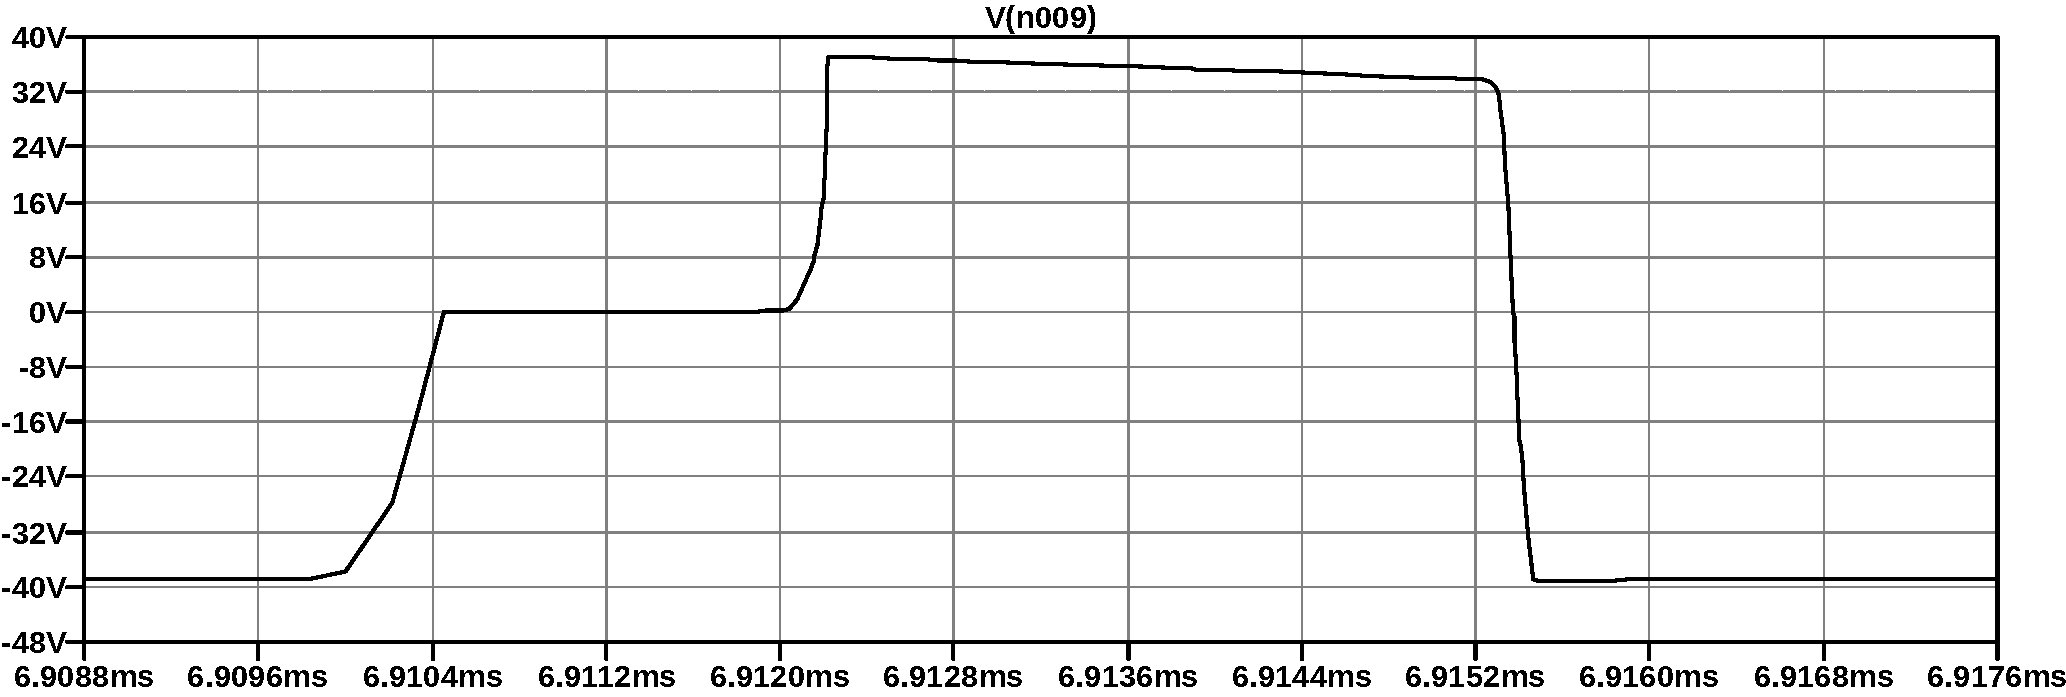
\includegraphics[width=\textwidth]{images/sim/20.pdf}
    \caption{Simulación de la tensión en el secundario del transformador de potencia}
    \label{fig:sim:20}
\end{figure}

% 5) Corriente en el primario %Del e70?

    % Medir la componente continua. IMPOSSIBLE
Las figuras \ref{fig:osc:24} muestra la corriente que circula por el primario del transformador de potencia. La figura \ref{fig:sim:12} muestra la simulación de la misma.

\begin{figure}[H]
    \centering
    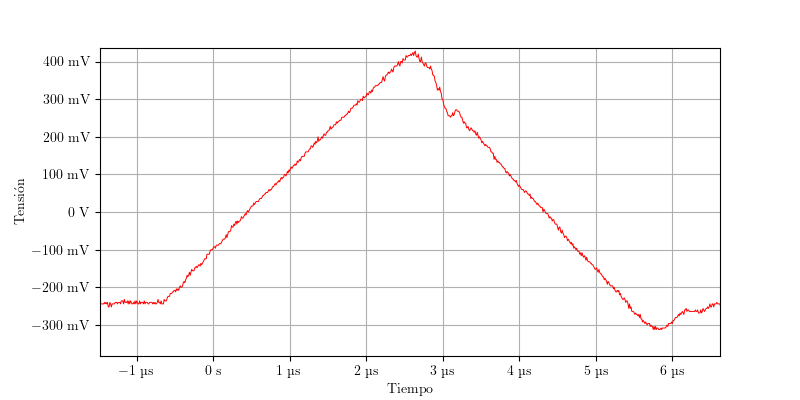
\includegraphics[width=0.8\textwidth]{images/capturas-osciloscopio/17-11-2022/24.png}
    \caption{Corriente en el primario del transformador de potencia}
    \label{fig:osc:24}
\end{figure}

\begin{figure}[H]
    \centering
    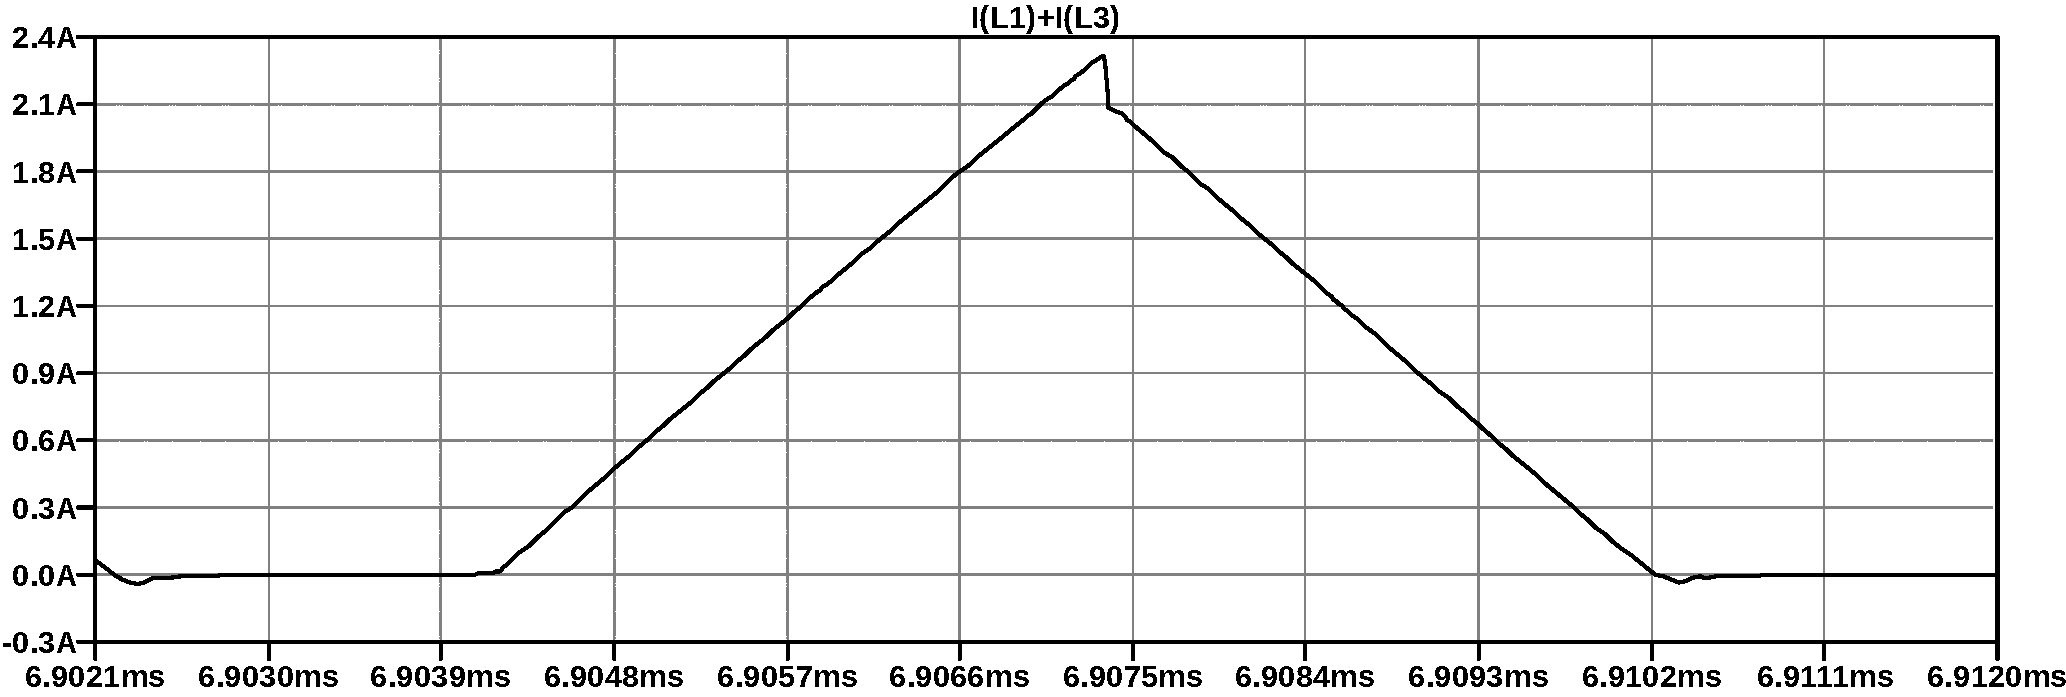
\includegraphics[width=\textwidth]{images/sim/12.pdf}
    \caption{Simulación de la corriente en el primario del transformador de potencia}
    \label{fig:sim:12}
\end{figure}

\subsubsection{Circuito de salida}
% 7) Corriente en el inductor junto con su ripple

La corriente por el inductor de salida se muestra en la figura \ref{fig:osc:66}. La figura \ref{fig:sim:13} muestra su simulación.

\begin{figure}[H]
    \centering
    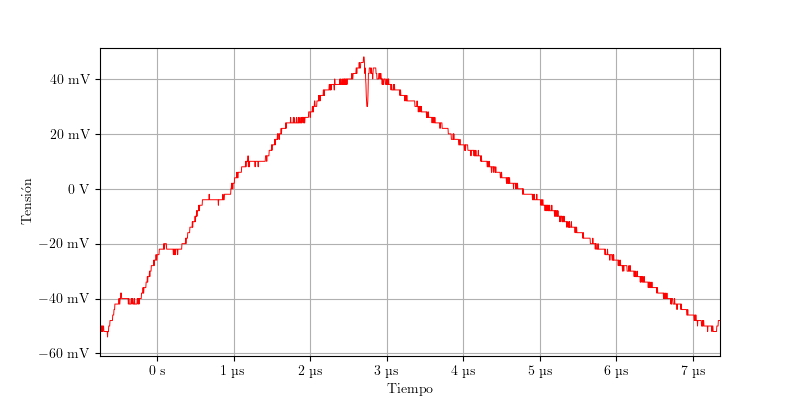
\includegraphics[width=0.8\textwidth]{images/capturas-osciloscopio/17-11-2022/66.png}
    \caption{Corriente en el inductor del filtro de salida}
    \label{fig:osc:66}
\end{figure}

\begin{figure}[H]
    \centering
    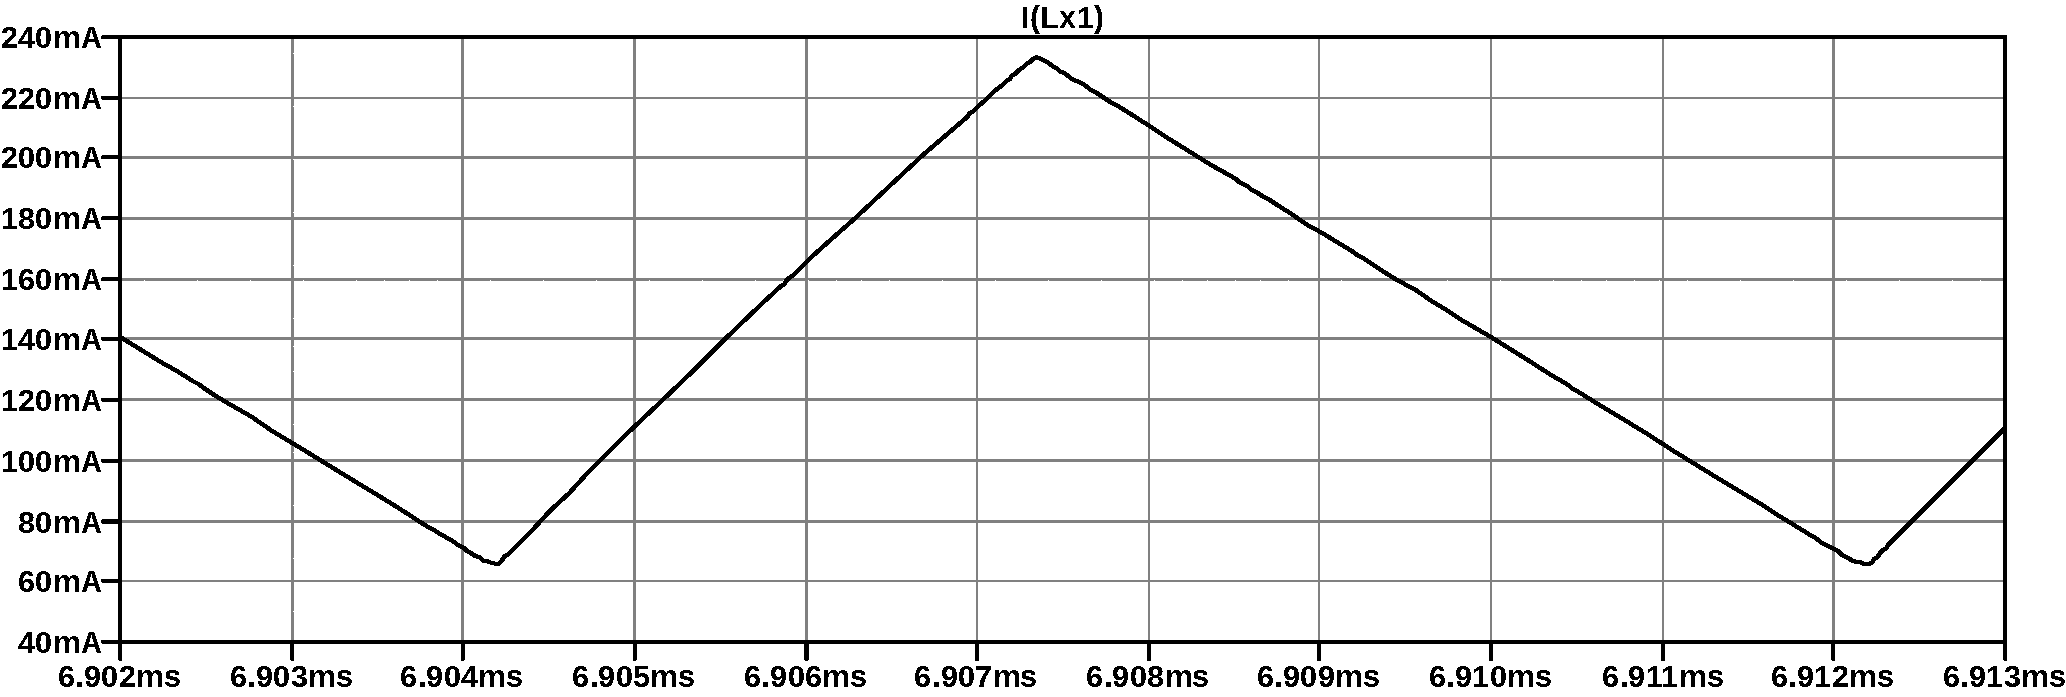
\includegraphics[width=\textwidth]{images/sim/13.pdf}
    \caption{Simulación de la corriente en el inductor del filtro de salida}
    \label{fig:sim:13}
\end{figure}

En las figuras \ref{fig:osc:67} y \ref{fig:sim:14ripple} se muestra la corriente por la resistencia de carga y su simulación, respectivamente. Se puede observar que el ripple obtenido es mayor al simulado.

La figura \ref{fig:sim:14} muestra la simulación de la corriente de salida durante el encendido.
% 8) Corriente de salida junto con su ripple 

    % Idealmente medir 1A-1.6A del modo elegido. 

\begin{figure}[H]
    \centering
    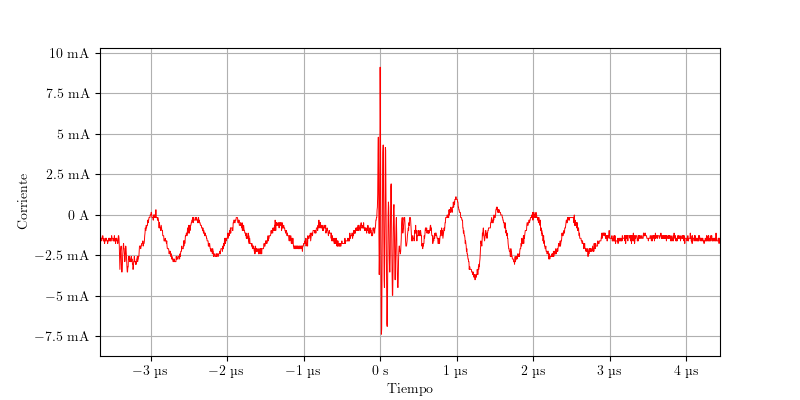
\includegraphics[width=0.8\textwidth]{images/capturas-osciloscopio/17-11-2022/67.png}
    \caption{Ripple de corriente por la carga}
    \label{fig:osc:67}
\end{figure}

\begin{figure}[H]
    \centering
    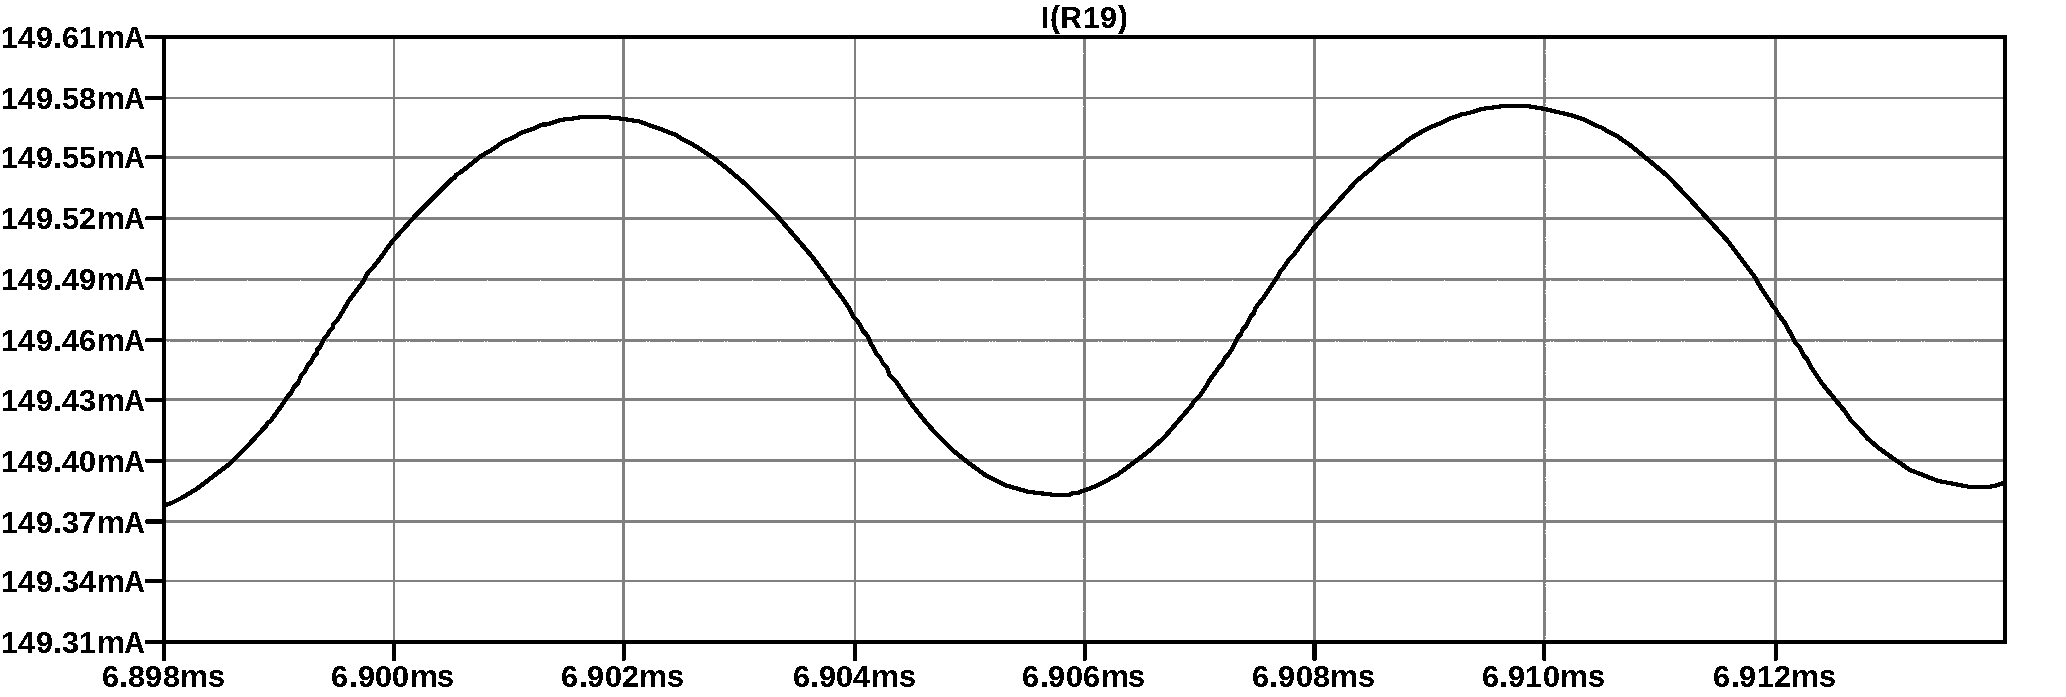
\includegraphics[width=\textwidth]{images/sim/14-ripple.pdf}
    \caption{Simulación del ripple de corriente por la carga}
    \label{fig:sim:14ripple}
\end{figure}

\begin{figure}[H]
    \centering
    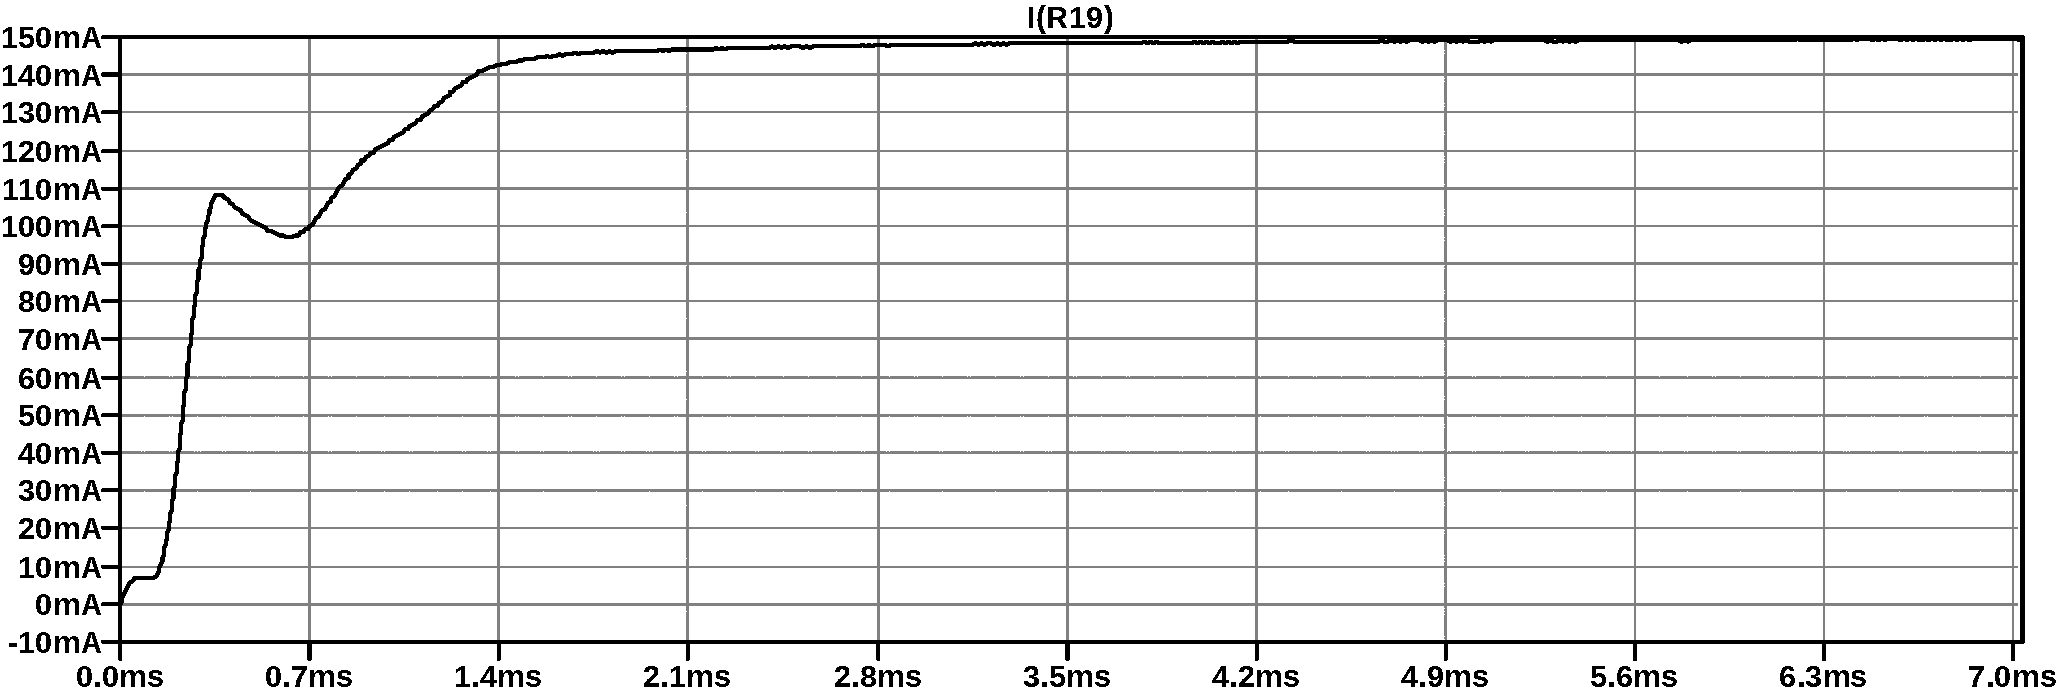
\includegraphics[width=\textwidth]{images/sim/14.pdf}
    \caption{Simulación de la corriente por la carga}
    \label{fig:sim:14}
\end{figure}

Análogamente, en las figuras \ref{fig:osc:58} y \ref{fig:sim:21ripple} se muestra el ripple de tensión en la salida salida y su simulación. En la figura \ref{fig:sim:21} se muestra la simulación de la tensión de salida durante el encendido.<
% 9) Tensión de salida junto con su ripple 

\begin{figure}[H]
    \centering
    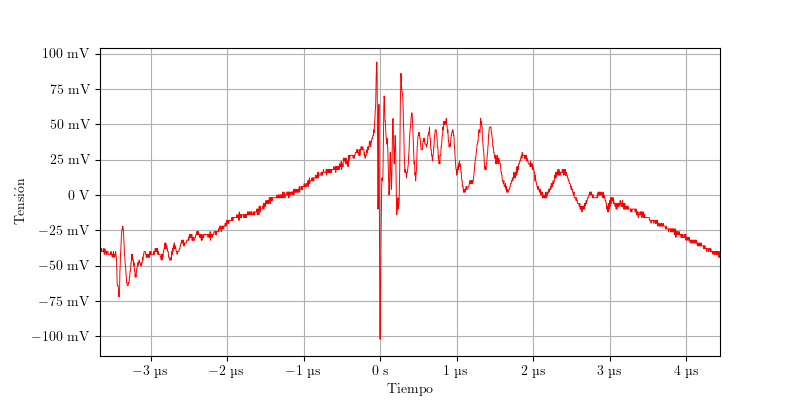
\includegraphics[width=0.8\textwidth]{images/capturas-osciloscopio/17-11-2022/58.png}
    \caption{Ripple de tensión en la carga}
    \label{fig:osc:58}
\end{figure}

\begin{figure}[H]
    \centering
    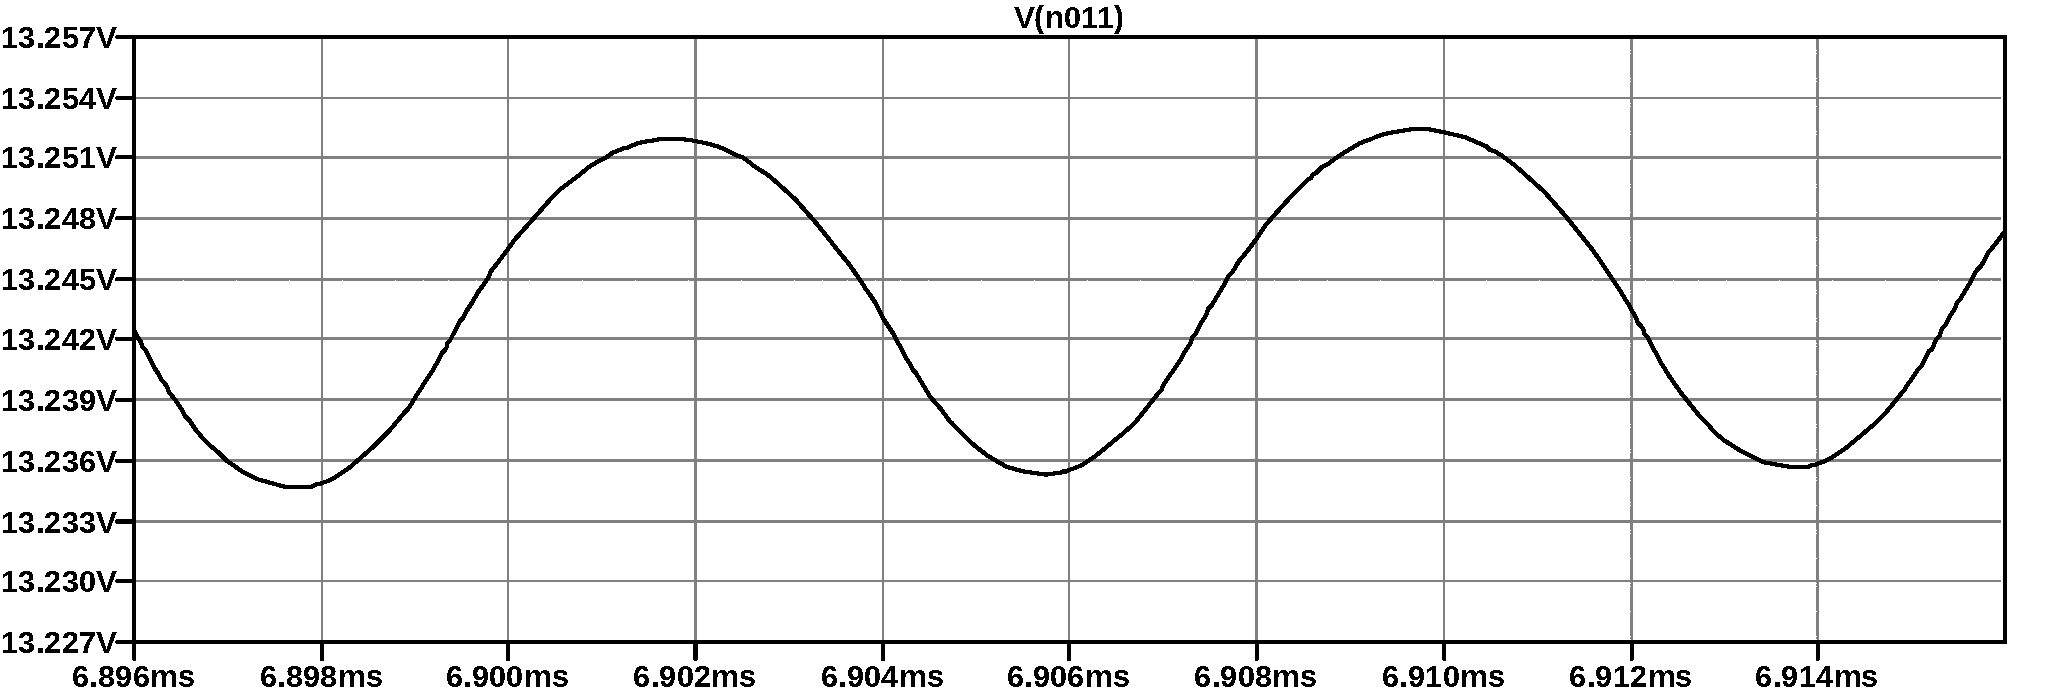
\includegraphics[width=\textwidth]{images/sim/21-ripple.pdf}
    \caption{Simulación del ripple de tensión en la carga}
    \label{fig:sim:21ripple}
\end{figure}

\begin{figure}[H]
    \centering
    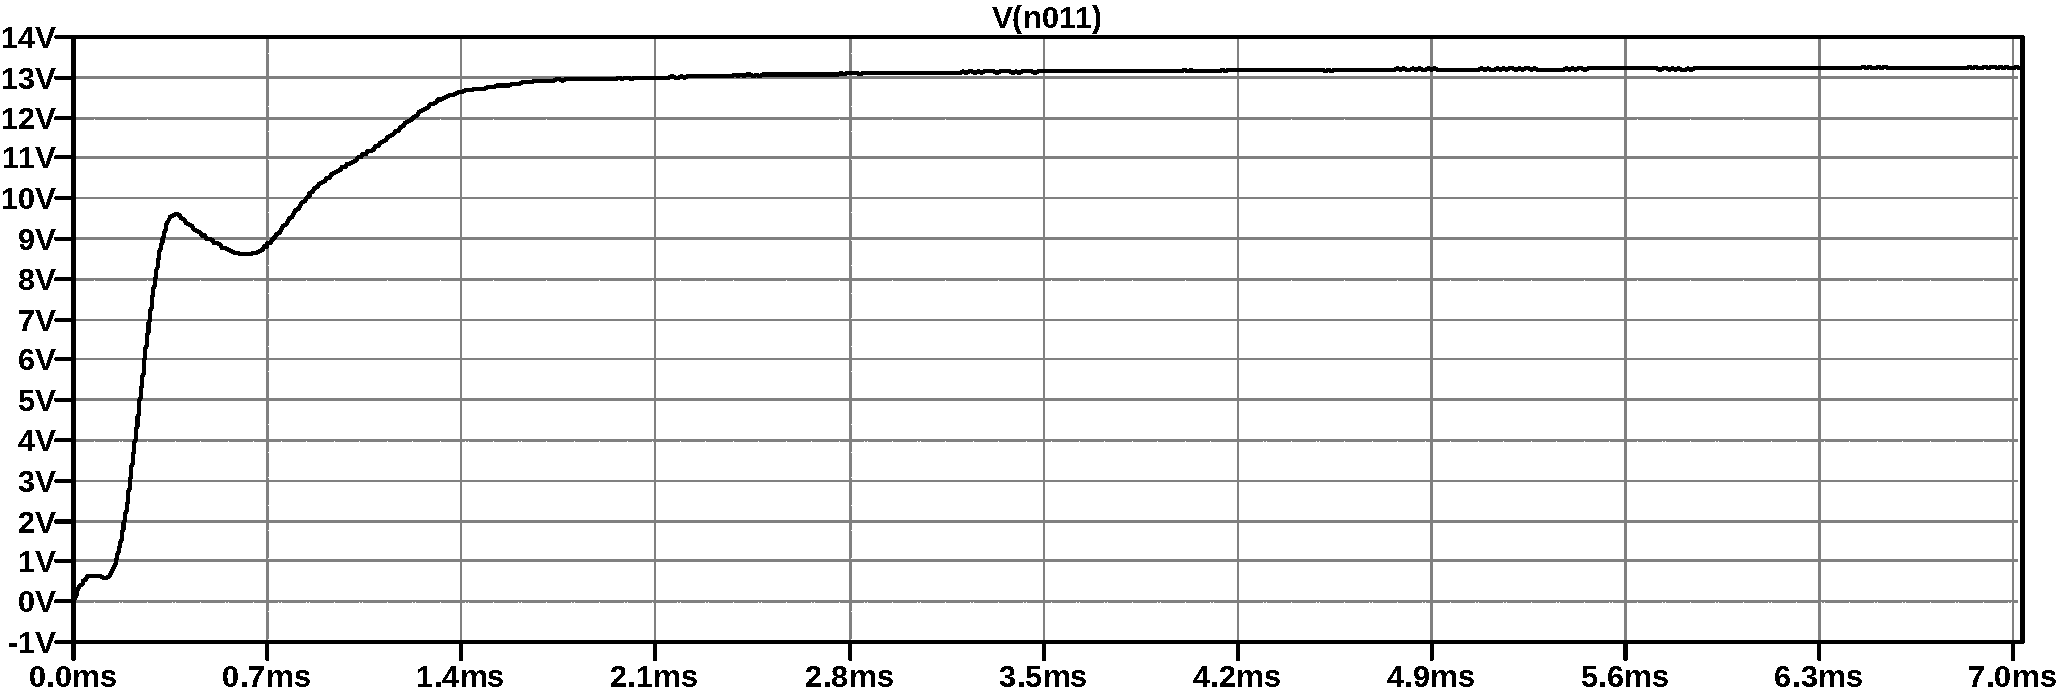
\includegraphics[width=\textwidth]{images/sim/21.pdf}
    \caption{Simulación de la tensión en la carga}
    \label{fig:sim:21}
\end{figure}

La tensión de salida no se mantiene estable ante variaciones en la carga con ciclo de trabajo y tensión de alimentación fija. 
Esto puede deberse a que se consideró el modelo ideal de todos los componentes del circuito al momento de realizar el análisis del convertidor. 

En la teoría analizada por la bibliografía se supone que todos los componentes del convertidor forward son ideales. 
Esto se evidencia en el simulador donde al utilizar modelos reales de los semiconductores se comienza a evidenciar como la tensión de salida varía levemente con la carga. 
Esta suposición realizada para simplificar el análisis lleva a tener diferencias en la práctica principalmente con el comportamiento de la tensión de salida. 
Ejemplos: resistencia del inductor del filtro de salida, pérdidas en los MOSFETs,
Se evidencia como ante el aumento de la corriente de carga la tensión de salida obtenida disminuye y se aleja del comportamiento semi-ideal del simulador. 
Como las pérdidas en todos los componentes aumentan con la corriente de carga. 
Es por ello que en la práctica los convertidores funcionan a lazo cerrado sensando la tensión o corriente de salida, y por medio de un sistema de realimentación ajustan el ciclo de trabajo para obtener una tensión de salida constante ante los cambios de carga o la tensión de entrada del convertidor.